\documentclass[11pt,a4paper]{article}

% Image mode: pdf.
% Image paths stay relative. In PDF mode, place same-basename PDF conversions
% of the chapter SVG files in the assets/ directory beside this source.

\usepackage{iftex}
\ifPDFTeX
  \PackageError{handout}{This template requires XeTeX or Tectonic}{Compile with xelatex or tectonic.}
\fi

\usepackage[a4paper,top=18mm,bottom=20mm,left=20mm,right=20mm,headsep=6mm]{geometry}
\usepackage{fontspec}
\usepackage{xeCJK}
\usepackage{amsmath}
\usepackage{unicode-math}

% Font settings are intentionally visible in the generated .tex file.
% These defaults target the macOS machine used for the released PDF.
% Change the family names when compiling on another system.
\setmainfont{Songti TC}
\setsansfont{Heiti TC}
\setmonofont{Menlo}
\setCJKmainfont{Songti TC}
\setCJKsansfont{Heiti TC}
\setCJKmonofont{Heiti TC}
\setmathfont{STIX Two Math}
\XeTeXlinebreaklocale "zh"
\XeTeXlinebreakskip=0pt plus 1pt

\usepackage{xcolor}
\definecolor{HandoutBlue}{HTML}{215A91}
\definecolor{HandoutBlueLight}{HTML}{EEF5FC}
\definecolor{HandoutGreen}{HTML}{39715A}
\definecolor{HandoutGreenLight}{HTML}{EFF8F3}
\definecolor{HandoutGold}{HTML}{8A641C}
\definecolor{HandoutGoldLight}{HTML}{FFF8E8}
\definecolor{HandoutInk}{HTML}{253142}
\definecolor{HandoutMuted}{HTML}{667085}

\usepackage{graphicx}
\makeatletter
% Pandoc 3 emits an accessibility `alt` key for raster/PDF images. Older
% graphicx releases do not know that key, so accept it without changing layout.
\@ifundefined{KV@Gin@alt}{\define@key{Gin}{alt}{}}{}
\newsavebox\pandoc@box
\newcommand*\pandocbounded[1]{%
  \sbox\pandoc@box{#1}%
  \Gscale@div\@tempa{\textheight}{\dimexpr\ht\pandoc@box+\dp\pandoc@box\relax}%
  \Gscale@div\@tempb{\linewidth}{\wd\pandoc@box}%
  \ifdim\@tempb\p@<\@tempa\p@\let\@tempa\@tempb\fi
  \ifdim\@tempa\p@<\p@\scalebox{\@tempa}{\usebox\pandoc@box}%
  \else\usebox{\pandoc@box}%
  \fi
}
\makeatother
\usepackage{float}
\floatplacement{figure}{H}
% Pandoc uses LTcaptype=none for uncaptioned longtables. The caption package
% expects that name to exist as a counter even though it is never displayed.
\newcounter{none}
\usepackage{caption}
\captionsetup[figure]{labelformat=empty,labelsep=none,font=small}

\usepackage{booktabs,longtable,array,calc}
\usepackage{etoolbox}
\makeatletter
\patchcmd\longtable{\par}{\if@noskipsec\mbox{}\fi\par}{}{}
\makeatother

\usepackage[most]{tcolorbox}
\tcbuselibrary{breakable,skins}
\newtcolorbox{HandoutLearningMap}{
  enhanced,breakable,colback=HandoutBlueLight,colframe=HandoutBlue,
  boxrule=0.8pt,arc=1.5mm,left=3mm,right=3mm,top=2mm,bottom=2mm,
  before skip=8pt,after skip=10pt
}
\newtcolorbox{HandoutWorkedExample}{
  enhanced,breakable,colback=HandoutGreenLight,colframe=HandoutGreen,
  boxrule=0.65pt,arc=1.5mm,left=3mm,right=3mm,top=2mm,bottom=2mm,
  before skip=8pt,after skip=10pt
}
\newtcolorbox{HandoutSelfCheck}{
  enhanced,breakable,colback=HandoutGoldLight,colframe=HandoutGold,
  boxrule=0.65pt,arc=1.5mm,left=3mm,right=3mm,top=2mm,bottom=2mm,
  before skip=8pt,after skip=10pt
}

\usepackage{titlesec}
\titleformat{\section}{\sffamily\bfseries\Large\color{HandoutBlue}}{}{0pt}{}
\titleformat{\subsection}{\sffamily\bfseries\large\color{HandoutInk}}{}{0pt}{}
\titleformat{\subsubsection}{\sffamily\bfseries\normalsize\color{HandoutInk}}{}{0pt}{}
\titlespacing*{\section}{0pt}{1.4em}{0.55em}
\titlespacing*{\subsection}{0pt}{1.15em}{0.45em}
\titlespacing*{\subsubsection}{0pt}{0.9em}{0.35em}
\setcounter{secnumdepth}{-\maxdimen}

\usepackage{hyperref}
\usepackage{bookmark}
\IfFileExists{xurl.sty}{\usepackage{xurl}}{}
\urlstyle{same}
\hypersetup{
  colorlinks=true,
  linkcolor=HandoutBlue,
  urlcolor=HandoutBlue,
  citecolor=HandoutBlue,
  pdftitle={數A4-2 空間中的平面與直線},
  pdfsubject={數學},
  pdfcreator={Pandoc with the HighSchooContent LaTeX template}
}

\setlength{\parindent}{0pt}
\setlength{\parskip}{0.55em plus 0.15em minus 0.1em}
\setlength{\emergencystretch}{3em}
\setlength{\LTpre}{0.5em}
\setlength{\LTpost}{0.5em}
\renewcommand{\arraystretch}{1.18}
\providecommand{\tightlist}{%
  \setlength{\itemsep}{0pt}\setlength{\parskip}{0pt}}
\pagestyle{plain}


\begin{document}

\begin{tcolorbox}[
  enhanced,colback=white,colframe=HandoutBlue,boxrule=1.1pt,arc=2mm,
  borderline west={3pt}{0pt}{HandoutBlue},left=5mm,right=4mm,top=4mm,bottom=4mm
]
{\sffamily\small\bfseries\color{HandoutBlue}學生講義}\par
{\sffamily\bfseries\LARGE\color{HandoutInk}數A4-2 空間中的平面與直線}\par
\vspace{0.35em}{\large 用方程式描述三維幾何，再由向量求交集、投影、角度與最短距離}\par
\vspace{0.45em}{\small\color{HandoutMuted}%
科目：數學
\quad 課程：普通高中數學A 第四冊
\quad 版本：學生版｜核心＋理解
\quad 校訂：2026-08-29
}\par
\vspace{0.25em}{\small\color{HandoutMuted}範圍：現行數學A主線}\par
\end{tcolorbox}


\begin{HandoutLearningMap}

\subsection{本章核心問題}\label{ux672cux7ae0ux6838ux5fc3ux554fux984c}

\begin{enumerate}
\def\labelenumi{\arabic{enumi}.}
\tightlist
\item
  \textbf{一個平面如何寫成方程式？}──平面上一點與法向量決定所有允許的位置。
\item
  \textbf{一條直線如何寫成方程式？}──直線上一點與方向向量決定參數移動路徑。
\item
  \textbf{怎麼判斷直線、平面的交集與角度？}──比較方向向量與法向量，再聯立參數。
\item
  \textbf{怎麼找投影與最短距離？}──最短連線沿著垂直方向；內積、外積與三重積提供計算工具。
\end{enumerate}

{藍色：現行核心}
{青綠：理解支援與用途}

\end{HandoutLearningMap}

\section{0. 方程式是三維空間的篩選條件}\label{ux65b9ux7a0bux5f0fux662fux4e09ux7dadux7a7aux9593ux7684ux7be9ux9078ux689dux4ef6}

點 \((x,y,z)\) 有三個可變坐標。一條獨立的一次方程式會限制一個自由度，通常留下二維的平面；兩條獨立平面方程式同時成立，通常留下它們的一維交線；再加一條獨立條件，通常決定一個交點。

另一種描述直線的方法是直接寫出移動規則：從固定點 \(A\) 出發，沿固定方向 \(\vec d\) 移動 \(t\) 倍，得到

\[
X=A+t\vec d.
\]

建築資訊模型用平面方程式描述牆面與樓板，以直線描述管線與樑柱；導航系統用參數 \(t\) 表示物體沿路徑的位置；三維掃描以投影找最近表面點。這些應用都在回答同一件事：某點是否符合幾何限制，以及符合限制的最近位置在哪裡。

\section{1. 平面方程式}\label{ux5e73ux9762ux65b9ux7a0bux5f0f}

\subsection{1.1 法向量與點法式}\label{ux6cd5ux5411ux91cfux8207ux9edeux6cd5ux5f0f}

與平面內所有方向垂直的非零向量稱為平面的法向量。設平面 \(E\) 通過

\[
A=(x_0,y_0,z_0),
\]

法向量為

\[
\vec n=(a,b,c)\ne\vec0.
\]

任取平面上一點 \(X=(x,y,z)\)，位移

\[
\overrightarrow{AX}=(x-x_0,y-y_0,z-z_0)
\]

位於平面內，因此與 \(\vec n\) 垂直：

\[
\vec n\cdot\overrightarrow{AX}=0.
\]

展開得到平面的點法式：

\[
\boxed{
a(x-x_0)+b(y-y_0)+c(z-z_0)=0
}.
\]

\begin{figure}
\centering
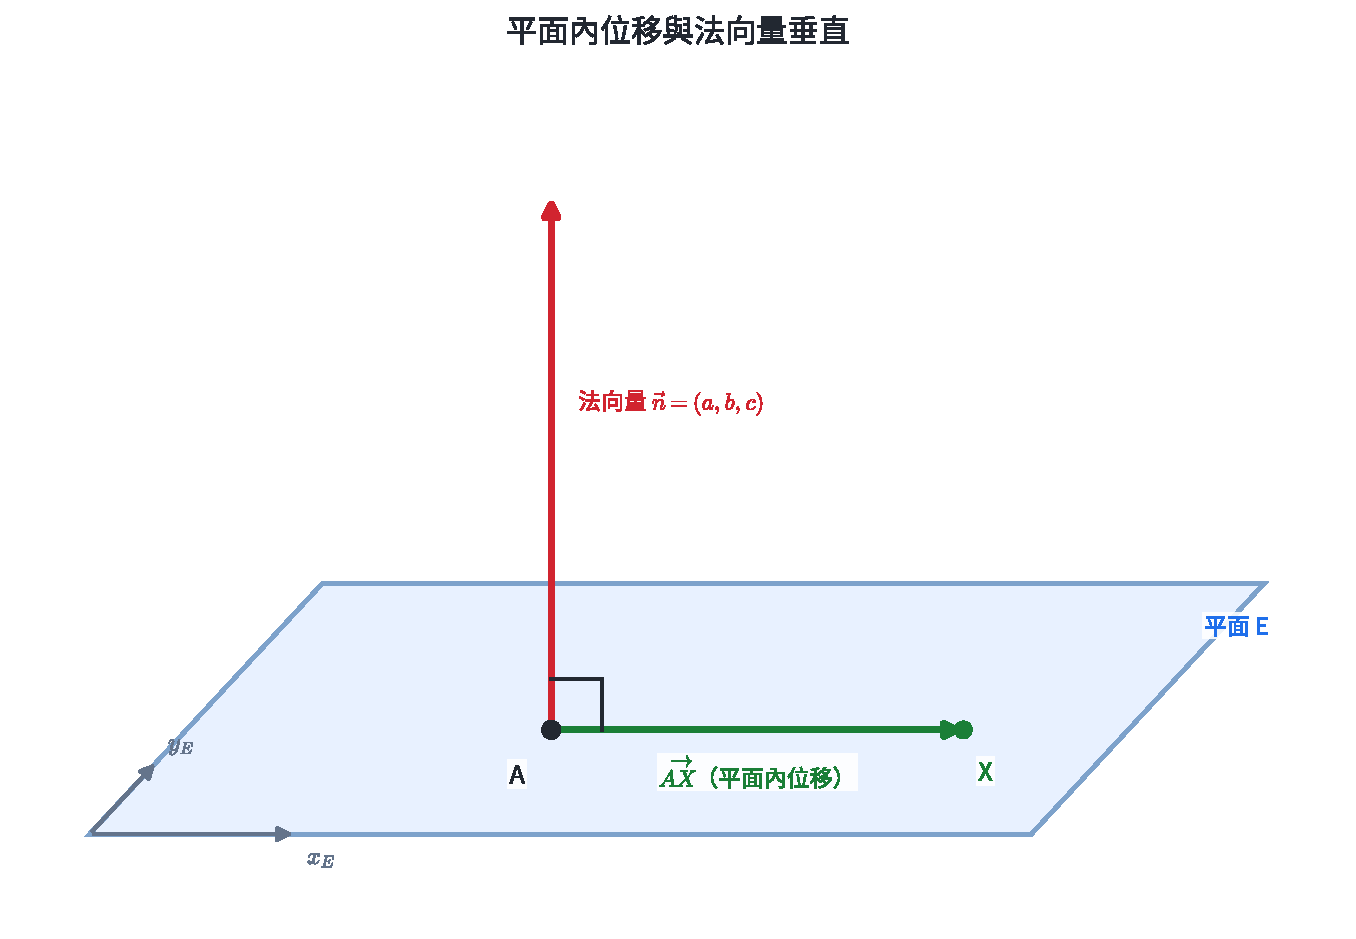
\includegraphics[width=0.84\linewidth,height=\textheight,keepaspectratio,alt={圖 1｜平面內的每一個位移都與法向量垂直；這個內積條件就是點法式。}]{assets/數A4-2-點法式與法向量.pdf}
\caption{圖 1｜平面內的每一個位移都與法向量垂直；這個內積條件就是點法式。}
\end{figure}

把常數整理，可寫成一般式

\[
\boxed{ax+by+cz+d=0},
\]

其中 \((a,b,c)\) 就是法向量。四個係數同乘非零常數仍表示同一平面；例如 \(x-2y+z=3\) 與 \(2x-4y+2z=6\) 的解集合完全相同。

法向量只決定朝向。要決定平面的位置，還需要平面上一點或常數項 \(d\)。

\subsection{1.2 由三點求平面}\label{ux7531ux4e09ux9edeux6c42ux5e73ux9762}

三個不共線點 \(A,B,C\) 決定唯一平面。先建立兩個不平行的平面內向量

\[
\overrightarrow{AB},\qquad\overrightarrow{AC},
\]

它們的外積

\[
\boxed{
\vec n=\overrightarrow{AB}\times\overrightarrow{AC}
}
\]

同時垂直兩個平面內方向，因此是法向量。接著把 \(\vec n\) 與任一點代入點法式。

若外積為零，三點共線，能通過它們的平面有無限多個；此時資料不足以決定唯一平面。

\subsection{1.3 截距式與坐標軸關係}\label{ux622aux8dddux5f0fux8207ux5750ux6a19ux8ef8ux95dcux4fc2}

若平面與 \(x,y,z\) 軸分別交於

\[
(p,0,0),\qquad(0,q,0),\qquad(0,0,r),
\]

而且 \(p,q,r\) 都非零，則平面可寫成

\[
\boxed{
\frac{x}{p}+\frac{y}{q}+\frac{z}{r}=1
}.
\]

逐一代入三個截距點都得到 \(1\)；由三個不共線點決定唯一平面，所以公式成立。

\begin{figure}
\centering
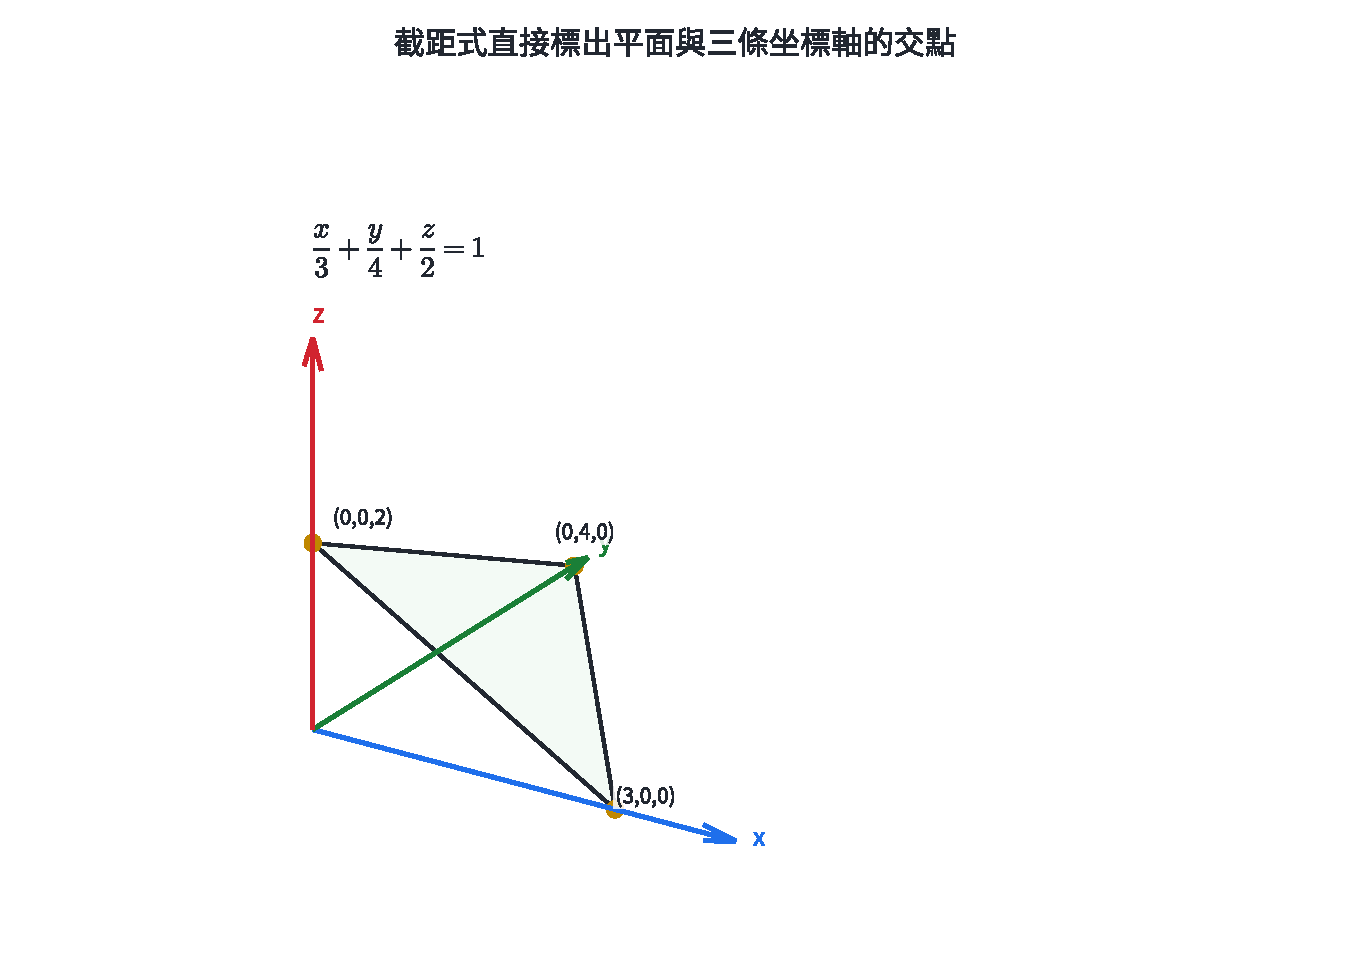
\includegraphics[width=0.82\linewidth,height=\textheight,keepaspectratio,alt={圖 2｜截距式的三個分母直接對應平面與三條坐標軸的交點。}]{assets/數A4-2-截距式.pdf}
\caption{圖 2｜截距式的三個分母直接對應平面與三條坐標軸的交點。}
\end{figure}

一般式的係數也能快速讀出與坐標軸、坐標平面的關係：

\begin{itemize}
\tightlist
\item
  \(x=k\) 的法向量平行 \(x\) 軸，所以平面垂直 \(x\) 軸、平行 \(yz\) 平面；
\item
  \(ax+by+d=0\) 沒有 \(z\) 項，法向量的 \(z\) 分量為 \(0\)，所以平面平行 \(z\) 軸；
\item
  通過原點的平面常數項為 \(0\)。
\end{itemize}

\subsection{法向量把整個平面的朝向濃縮成三個數}\label{ux6cd5ux5411ux91cfux628aux6574ux500bux5e73ux9762ux7684ux671dux5411ux6fc3ux7e2eux6210ux4e09ux500bux6578}

平面上有無限多個方向，直接逐一描述並不實用。法向量垂直所有平面內方向，只要三個分量就能代表整個平面的朝向。

電腦圖學用法向量判斷表面面向光源的程度；工程軟體用法向量檢查兩個零件面是否平行或垂直；測量資料擬合平面後，也以法向量記錄坡面朝向。

\begin{HandoutWorkedExample}

\subsection{完整示範｜由一點與法向量建立平面}\label{ux5b8cux6574ux793aux7bc4ux7531ux4e00ux9edeux8207ux6cd5ux5411ux91cfux5efaux7acbux5e73ux9762}

平面通過 \(A=(1,3,-2)\)，法向量為 \(\vec n=(2,-1,2)\)。求平面方程式。

代入點法式：

\[
2(x-1)-(y-3)+2(z+2)=0.
\]

展開：

\[
2x-y+2z+5=0.
\]

因此

\[
\boxed{E:2x-y+2z+5=0}.
\]

核對 \(A\)：\(2(1)-3+2(-2)+5=0\)；一般式前三個係數也正好是指定法向量。

\end{HandoutWorkedExample}

\begin{HandoutWorkedExample}

\subsection{完整示範｜由三個截距點求平面}\label{ux5b8cux6574ux793aux7bc4ux7531ux4e09ux500bux622aux8dddux9edeux6c42ux5e73ux9762}

平面通過

\[
A=(1,0,0),\quad B=(0,2,0),\quad C=(0,0,3).
\]

三點分別是 \(x,y,z\) 軸截距，可直接寫成

\[
\boxed{x+\frac y2+\frac z3=1}.
\]

乘以 \(6\) 得一般式

\[
\boxed{6x+3y+2z-6=0}.
\]

以外積核對：

\[
\overrightarrow{AB}=(-1,2,0),
\qquad
\overrightarrow{AC}=(-1,0,3),
\]

\[
\overrightarrow{AB}\times\overrightarrow{AC}
=(6,3,2),
\]

與一般式的法向量一致。

\end{HandoutWorkedExample}

\begin{HandoutWorkedExample}

\subsection{完整示範｜包含一條坐標軸的平面}\label{ux5b8cux6574ux793aux7bc4ux5305ux542bux4e00ux689dux5750ux6a19ux8ef8ux7684ux5e73ux9762}

求包含 \(y\) 軸且通過 \(P=(2,3,-1)\) 的平面。

設一般式為

\[
ax+by+cz+d=0.
\]

\(y\) 軸上每一點 \((0,t,0)\) 都在平面上，所以對所有 \(t\)，

\[
bt+d=0.
\]

因此 \(b=0\)、\(d=0\)。再代入 \(P\)：

\[
2a-c=0.
\]

可取 \(a=1,c=2\)，得到

\[
\boxed{x+2z=0}.
\]

方程式沒有 \(y\) 項，表示沿 \(y\) 方向移動仍留在平面內，符合包含 \(y\) 軸的幾何條件。

\end{HandoutWorkedExample}

\begin{HandoutSelfCheck}

\subsection{節末練習｜平面方程式}\label{ux7bc0ux672bux7df4ux7fd2ux5e73ux9762ux65b9ux7a0bux5f0f}

\begin{enumerate}
\def\labelenumi{\arabic{enumi}.}
\tightlist
\item
  寫出平面 \(3x-2y+6z-5=0\) 的一個法向量，並判斷點 \((1,2,1)\) 是否在平面上。
\item
  求通過 \(A=(2,-1,3)\)、法向量為 \((1,2,-2)\) 的平面方程式。
\item
  求通過 \(A=(0,0,0)\)、\(B=(1,2,0)\)、\(C=(0,1,3)\) 的平面方程式。
\item
  一平面在 \(x,y,z\) 軸的截距分別為 \(2,-3,6\)。寫出截距式與一般式。
\item
  求包含 \(z\) 軸且通過 \(P=(2,-1,4)\) 的平面方程式。
\item
  平面 \(E\) 平行 \(z\) 軸，並通過 \(A=(1,0,2)\)、\(B=(0,2,-1)\)。求 \(E\)。
\end{enumerate}

\textbf{解答}

\begin{enumerate}
\def\labelenumi{\arabic{enumi}.}
\tightlist
\item
  法向量可取 \((3,-2,6)\)。代入點得 \(3-4+6-5=0\)，所以該點在平面上。
\item
  \((x-2)+2(y+1)-2(z-3)=0\)，整理得 \(\boxed{x+2y-2z+6=0}\)。
\item
  \(\overrightarrow{AB}=(1,2,0)\)、\(\overrightarrow{AC}=(0,1,3)\)，外積為 \((6,-3,1)\)。平面通過原點，所以 \(\boxed{6x-3y+z=0}\)。
\item
  截距式為 \(x/2-y/3+z/6=1\)；乘以 \(6\) 得 \(\boxed{3x-2y+z-6=0}\)。
\item
  包含 \(z\) 軸使方程式只有 \(x,y\) 項且常數為 \(0\)。代入 \(P\) 得 \(2a-b=0\)，可取 \(a=1,b=2\)，所以 \(\boxed{x+2y=0}\)。
\item
  平行 \(z\) 軸表示 \(z\) 方向在平面內。另取 \(\overrightarrow{AB}=(-1,2,-3)\)，與 \((0,0,1)\) 外積可得法向量 \((2,1,0)\)。代入 \(A\) 得 \(\boxed{2x+y-2=0}\)。
\end{enumerate}

\end{HandoutSelfCheck}

\section{2. 平面的夾角、投影與距離}\label{ux5e73ux9762ux7684ux593eux89d2ux6295ux5f71ux8207ux8dddux96e2}

\subsection{2.1 兩平面的夾角}\label{ux5169ux5e73ux9762ux7684ux593eux89d2}

設平面

\[
E_1:a_1x+b_1y+c_1z+d_1=0,
\]

\[
E_2:a_2x+b_2y+c_2z+d_2=0,
\]

法向量分別為

\[
\vec n_1=(a_1,b_1,c_1),
\qquad
\vec n_2=(a_2,b_2,c_2).
\]

兩平面的銳夾角等於兩法向量的銳夾角，因此

\[
\boxed{
\cos\theta
=\frac{|\vec n_1\cdot\vec n_2|}
{|\vec n_1|\,|\vec n_2|}
},
\qquad0^\circ\le\theta\le90^\circ.
\]

絕對值把法向量的正反方向視為同一平面朝向。

\begin{figure}
\centering
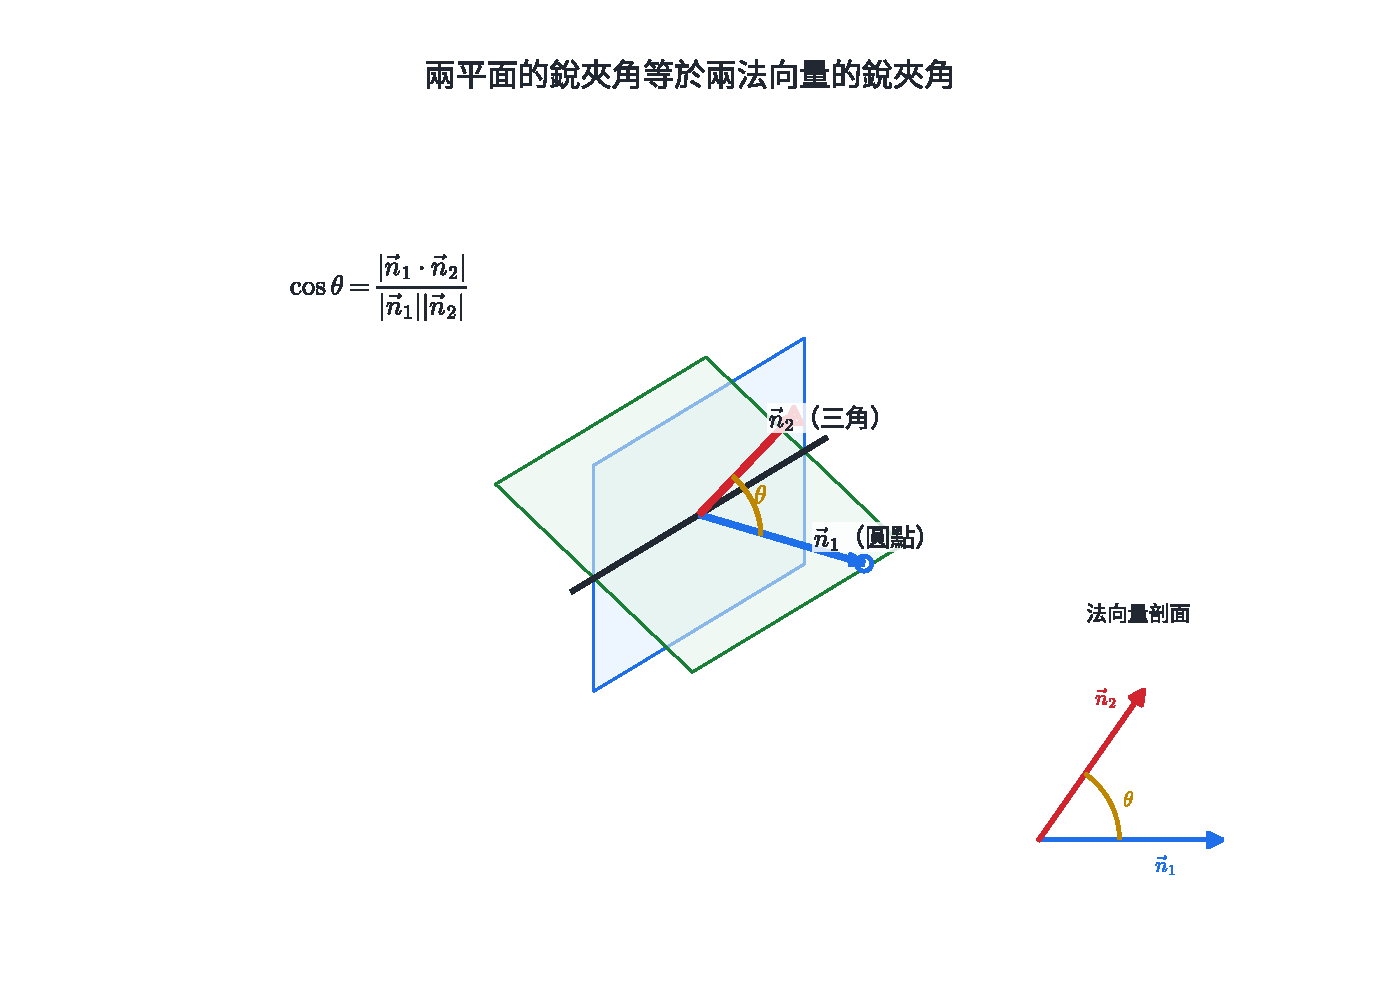
\includegraphics[width=0.84\linewidth,height=\textheight,keepaspectratio,alt={圖 3｜兩平面的交線同時垂直兩個法向量；銳二面角可由兩法向量的銳角求得。}]{assets/數A4-2-兩平面夾角.pdf}
\caption{圖 3｜兩平面的交線同時垂直兩個法向量；銳二面角可由兩法向量的銳角求得。}
\end{figure}

由法向量可直接判斷：

\[
\boxed{E_1\parallel E_2\iff\vec n_1\parallel\vec n_2},
\]

\[
\boxed{E_1\perp E_2\iff\vec n_1\cdot\vec n_2=0}.
\]

法向量平行時，兩平面可能平行或重合；再檢查一個平面上的點是否也滿足另一方程式即可區分。

\subsection{2.2 點到平面的距離與投影點}\label{ux9edeux5230ux5e73ux9762ux7684ux8dddux96e2ux8207ux6295ux5f71ux9ede}

設點 \(P=(x_0,y_0,z_0)\)，平面

\[
E:ax+by+cz+d=0,
\]

法向量 \(\vec n=(a,b,c)\)。取平面上任一點 \(A\)，\(\overrightarrow{AP}\) 沿法向量的投影長為

\[
\frac{|\overrightarrow{AP}\cdot\vec n|}{|\vec n|}.
\]

因 \(A\) 滿足 \(aA_x+bA_y+cA_z+d=0\)，分子整理成 \(|ax_0+by_0+cz_0+d|\)，得到

\[
\boxed{
d(P,E)=
\frac{|ax_0+by_0+cz_0+d|}{\sqrt{a^2+b^2+c^2}}
}.
\]

\begin{figure}
\centering
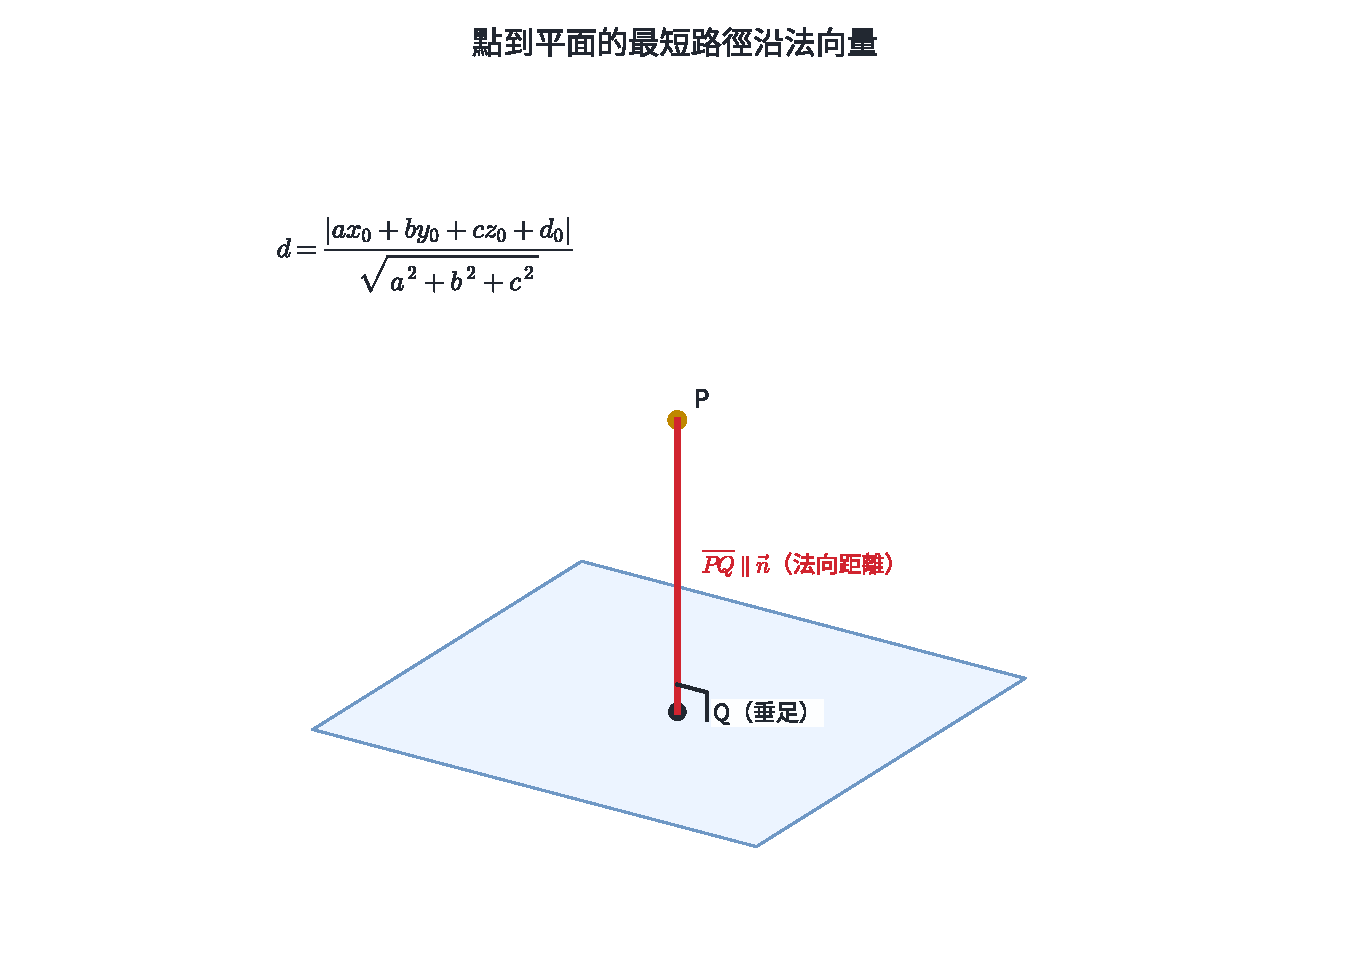
\includegraphics[width=0.82\linewidth,height=\textheight,keepaspectratio,alt={圖 4｜點到平面的最短線段沿法向量，終點就是正射影。}]{assets/數A4-2-點到平面距離.pdf}
\caption{圖 4｜點到平面的最短線段沿法向量，終點就是正射影。}
\end{figure}

令

\[
F(P)=ax_0+by_0+cz_0+d.
\]

從 \(P\) 沿法向量移到投影點 \(Q\)：

\[
Q=P-t\vec n.
\]

把 \(Q\) 代入平面方程式，得到

\[
F(P)-t|\vec n|^2=0,
\]

所以

\[
\boxed{
Q=P-\frac{F(P)}{|\vec n|^2}\vec n
}.
\]

點 \(P\) 關於平面 \(E\) 的對稱點 \(P'\) 以 \(Q\) 為中點：

\[
\boxed{P'=2Q-P}.
\]

\subsection{2.3 兩平行平面的距離}\label{ux5169ux5e73ux884cux5e73ux9762ux7684ux8dddux96e2}

兩平行平面須先寫成完全相同的法向係數：

\[
E_1:ax+by+cz+d_1=0,
\]

\[
E_2:ax+by+cz+d_2=0.
\]

任取 \(E_1\) 上一點，代入 \(E_2\) 的距離公式，可得

\[
\boxed{
d(E_1,E_2)=
\frac{|d_1-d_2|}{\sqrt{a^2+b^2+c^2}}
}.
\]

\begin{figure}
\centering
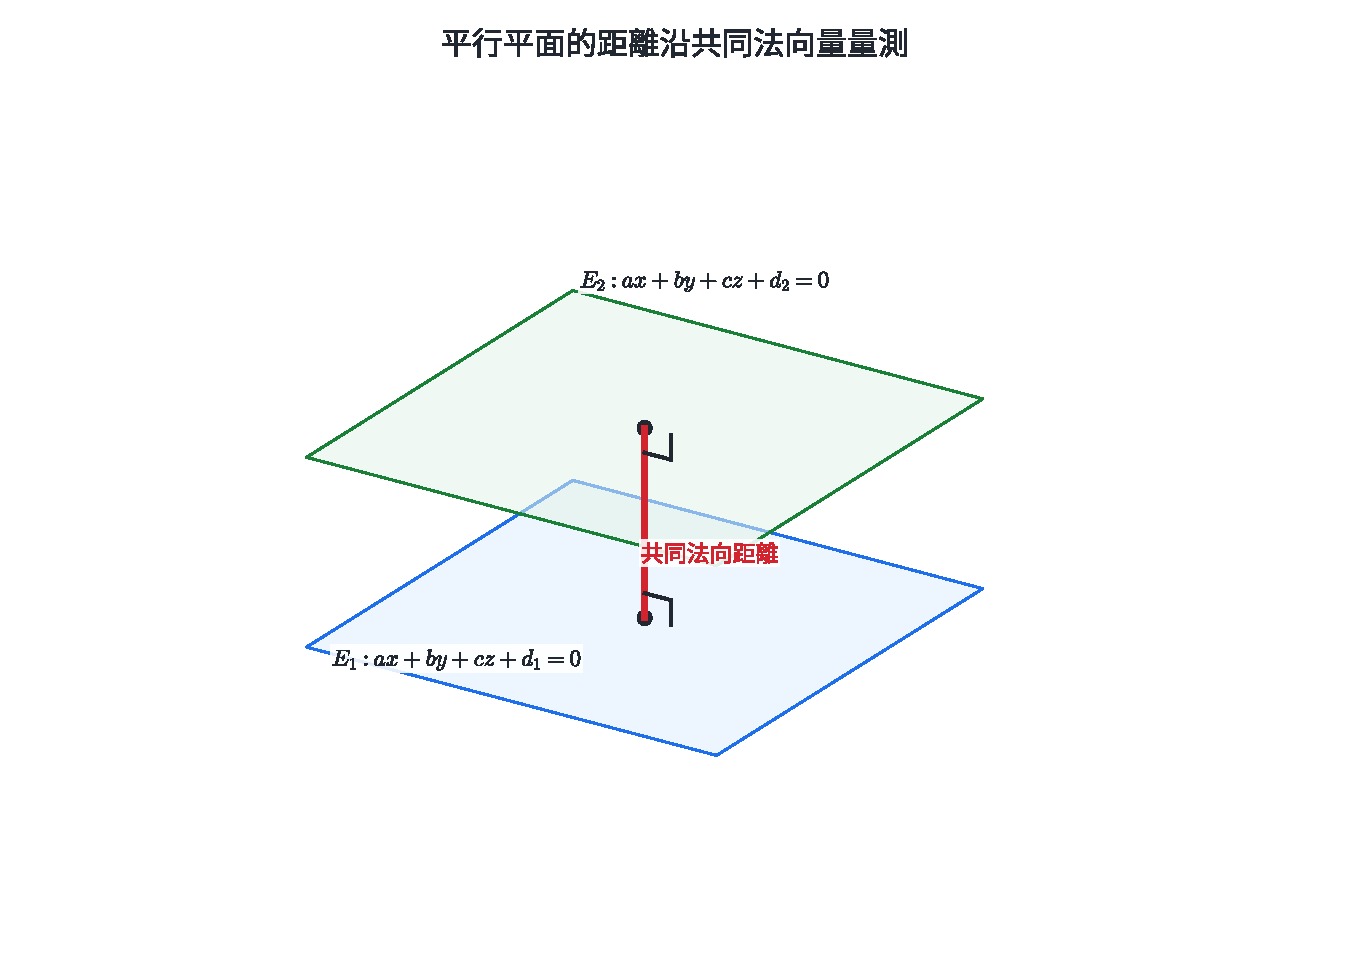
\includegraphics[width=0.82\linewidth,height=\textheight,keepaspectratio,alt={圖 5｜平行平面共享法向量，平面間距離就是沿共同法向量的固定長度。}]{assets/數A4-2-平行平面距離.pdf}
\caption{圖 5｜平行平面共享法向量，平面間距離就是沿共同法向量的固定長度。}
\end{figure}

若兩式的前三個係數成比例，先把整條方程式同乘或同除，使 \((a,b,c)\) 完全一致，再比較常數項。

\begin{HandoutWorkedExample}

\subsection{完整示範｜兩平面的銳夾角}\label{ux5b8cux6574ux793aux7bc4ux5169ux5e73ux9762ux7684ux92b3ux593eux89d2}

求

\[
E_1:2x-y+2z=3,
\qquad
E_2:x+2y-2z=4
\]

的銳夾角。

法向量為

\[
\vec n_1=(2,-1,2),
\qquad
\vec n_2=(1,2,-2).
\]

\[
\vec n_1\cdot\vec n_2=2-2-4=-4,
\qquad
|\vec n_1|=|\vec n_2|=3.
\]

所以

\[
\cos\theta=\frac{|-4|}{3\cdot3}=\frac49,
\]

\[
\boxed{\theta=\cos^{-1}\!\left(\frac49\right)\approx63.6^\circ}.
\]

\end{HandoutWorkedExample}

\begin{HandoutWorkedExample}

\subsection{完整示範｜點到平面的距離、投影與對稱}\label{ux5b8cux6574ux793aux7bc4ux9edeux5230ux5e73ux9762ux7684ux8dddux96e2ux6295ux5f71ux8207ux5c0dux7a31}

點 \(P=(1,-2,3)\)，平面

\[
E:2x-2y+z-5=0.
\]

法向量 \(\vec n=(2,-2,1)\)，\(|\vec n|=3\)。先算

\[
F(P)=2(1)-2(-2)+3-5=4.
\]

距離為

\[
\boxed{d(P,E)=\frac43}.
\]

投影點：

\[
Q=P-\frac4{9}(2,-2,1)
=\boxed{\left(\frac19,-\frac{10}{9},\frac{23}{9}\right)}.
\]

代回平面：

\[
\frac29+\frac{20}{9}+\frac{23}{9}-5=0.
\]

對稱點為

\[
P'=2Q-P
=\boxed{\left(-\frac79,-\frac29,\frac{19}{9}\right)}.
\]

\(Q\) 是 \(PP'\) 的中點，且 \(PP'\) 平行法向量。

\end{HandoutWorkedExample}

\begin{HandoutWorkedExample}

\subsection{完整示範｜係數先正規化再求平行平面距離}\label{ux5b8cux6574ux793aux7bc4ux4fc2ux6578ux5148ux6b63ux898fux5316ux518dux6c42ux5e73ux884cux5e73ux9762ux8dddux96e2}

求

\[
E_1:2x-y+2z-3=0,
\]

\[
E_2:4x-2y+4z+6=0
\]

的距離。

第二式除以 \(2\)：

\[
E_2:2x-y+2z+3=0.
\]

兩平面法向量相同，距離為

\[
d=\frac{|(-3)-3|}{\sqrt{2^2+(-1)^2+2^2}}
=\frac6{3}
=\boxed2.
\]

\end{HandoutWorkedExample}

\begin{HandoutSelfCheck}

\subsection{節末練習｜平面夾角與距離}\label{ux7bc0ux672bux7df4ux7fd2ux5e73ux9762ux593eux89d2ux8207ux8dddux96e2}

\begin{enumerate}
\def\labelenumi{\arabic{enumi}.}
\tightlist
\item
  判斷 \(E_1:x+2y-2z=1\) 與 \(E_2:2x+4y-4z=7\) 的關係。
\item
  求平面 \(x+y+z=1\) 與 \(x-y=2\) 的銳夾角。
\item
  求點 \(P=(2,-1,4)\) 到平面 \(2x+y-2z+3=0\) 的距離。
\item
  求點 \(P=(2,0,1)\) 在平面 \(x-2y+2z-1=0\) 上的投影點與對稱點。
\item
  求平面 \(x-2y+2z-3=0\) 與 \(3x-6y+6z+9=0\) 的距離。
\item
  求通過原點、且平行於 \(2x-y+2z=5\) 的平面。
\end{enumerate}

\textbf{解答}

\begin{enumerate}
\def\labelenumi{\arabic{enumi}.}
\tightlist
\item
  法向量成比例；把第二式除以 \(2\) 得 \(x+2y-2z=7/2\)，常數不同，所以兩平面平行。
\item
  法向量 \((1,1,1)\)、\((1,-1,0)\) 的內積為 \(0\)，所以兩平面垂直，夾角 \(90^\circ\)。
\item
  分子 \(|4-1-8+3|=2\)，分母為 \(3\)，所以距離為 \(\boxed{2/3}\)。
\item
  \(F(P)=2+2-1=3\)，\(|\vec n|^2=9\)。投影點 \(Q=P-\tfrac13(1,-2,2)=(5/3,2/3,1/3)\)；對稱點 \(P'=2Q-P=(4/3,4/3,-1/3)\)。
\item
  第二式除以 \(3\) 得 \(x-2y+2z+3=0\)。距離為 \(|{-3}-3|/3=\boxed2\)。
\item
  平行平面沿用法向量 \((2,-1,2)\)；通過原點使常數為 \(0\)，所以 \(\boxed{2x-y+2z=0}\)。
\end{enumerate}

\end{HandoutSelfCheck}

\section{3. 空間直線方程式}\label{ux7a7aux9593ux76f4ux7ddaux65b9ux7a0bux5f0f}

\subsection{3.1 向量式與參數式}\label{ux5411ux91cfux5f0fux8207ux53c3ux6578ux5f0f}

一條直線由線上一點

\[
A=(x_0,y_0,z_0)
\]

與非零方向向量

\[
\vec d=(a,b,c)
\]

決定。直線上任一點 \(X=(x,y,z)\) 都滿足

\[
\boxed{X=A+t\vec d},\qquad t\in\mathbb R.
\]

逐分量寫成參數式：

\[
\boxed{
\begin{cases}
x=x_0+at,\\
y=y_0+bt,\\
z=z_0+ct,
\end{cases}
\qquad t\in\mathbb R
}.
\]

參數 \(t\) 是有向移動倍數。\(t=0\) 位於基準點 \(A\)；\(t>0\) 沿 \(\vec d\) 前進；\(t<0\) 沿反方向前進。

\begin{figure}
\centering
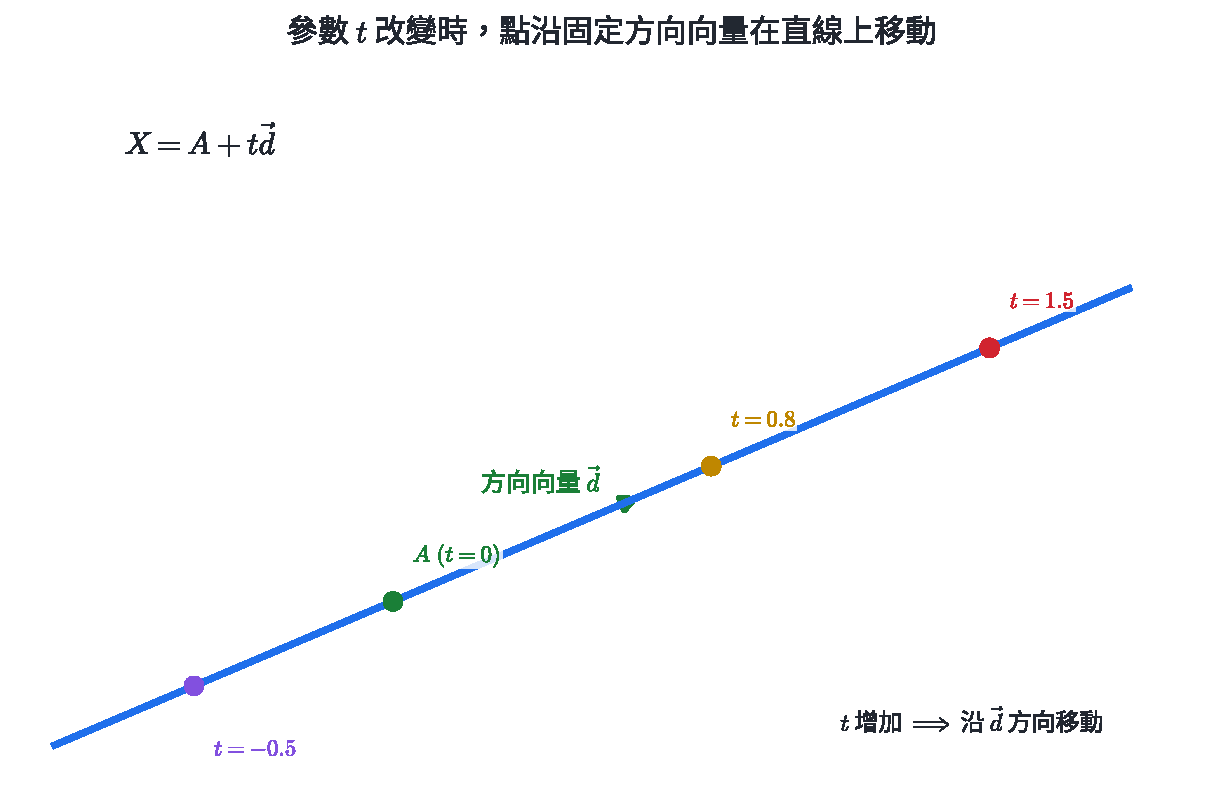
\includegraphics[width=0.84\linewidth,height=\textheight,keepaspectratio,alt={圖 6｜參數改變時，點從基準點沿方向向量在同一直線上移動。}]{assets/數A4-2-直線參數式.pdf}
\caption{圖 6｜參數改變時，點從基準點沿方向向量在同一直線上移動。}
\end{figure}

同一直線可選不同基準點，也可把方向向量乘任意非零常數，所以方程式不唯一。判斷是否為同一直線要比較解集合，而非比較外觀。

\subsection{3.2 比例式}\label{ux6bd4ux4f8bux5f0f}

若方向向量三個分量 \(a,b,c\) 都非零，消去參數 \(t\) 可得比例式：

\[
\boxed{
\frac{x-x_0}{a}
=\frac{y-y_0}{b}
=\frac{z-z_0}{c}
}.
\]

若某個方向分量為 \(0\)，相應坐標保持固定。例如方向向量 \((2,0,-1)\) 的直線寫成

\[
\frac{x-x_0}{2}
=\frac{z-z_0}{-1},
\qquad y=y_0.
\]

固定坐標比寫成分母 \(0\) 更能準確表達幾何條件。

\subsection{3.3 通過兩點的直線}\label{ux901aux904eux5169ux9edeux7684ux76f4ux7dda}

不同兩點 \(P,Q\) 決定唯一直線，方向向量可取

\[
\boxed{\vec d=Q-P}.
\]

線段 \(PQ\) 上的點可用 \(0\le t\le1\)：

\[
X=P+t(Q-P).
\]

\(t\) 超出 \([0,1]\) 時，點位於線段外的延長線。

\subsection{3.4 兩個平面的交線}\label{ux5169ux500bux5e73ux9762ux7684ux4ea4ux7dda}

兩個不平行平面

\[
E_1:\vec n_1\cdot X=d_1,
\qquad
E_2:\vec n_2\cdot X=d_2
\]

的交線方向同時垂直 \(\vec n_1,\vec n_2\)，所以可取

\[
\boxed{
\vec d=\vec n_1\times\vec n_2
}.
\]

再聯立兩個平面方程式找一個公共點 \(A\)，交線就是 \(X=A+t\vec d\)。

\begin{figure}
\centering
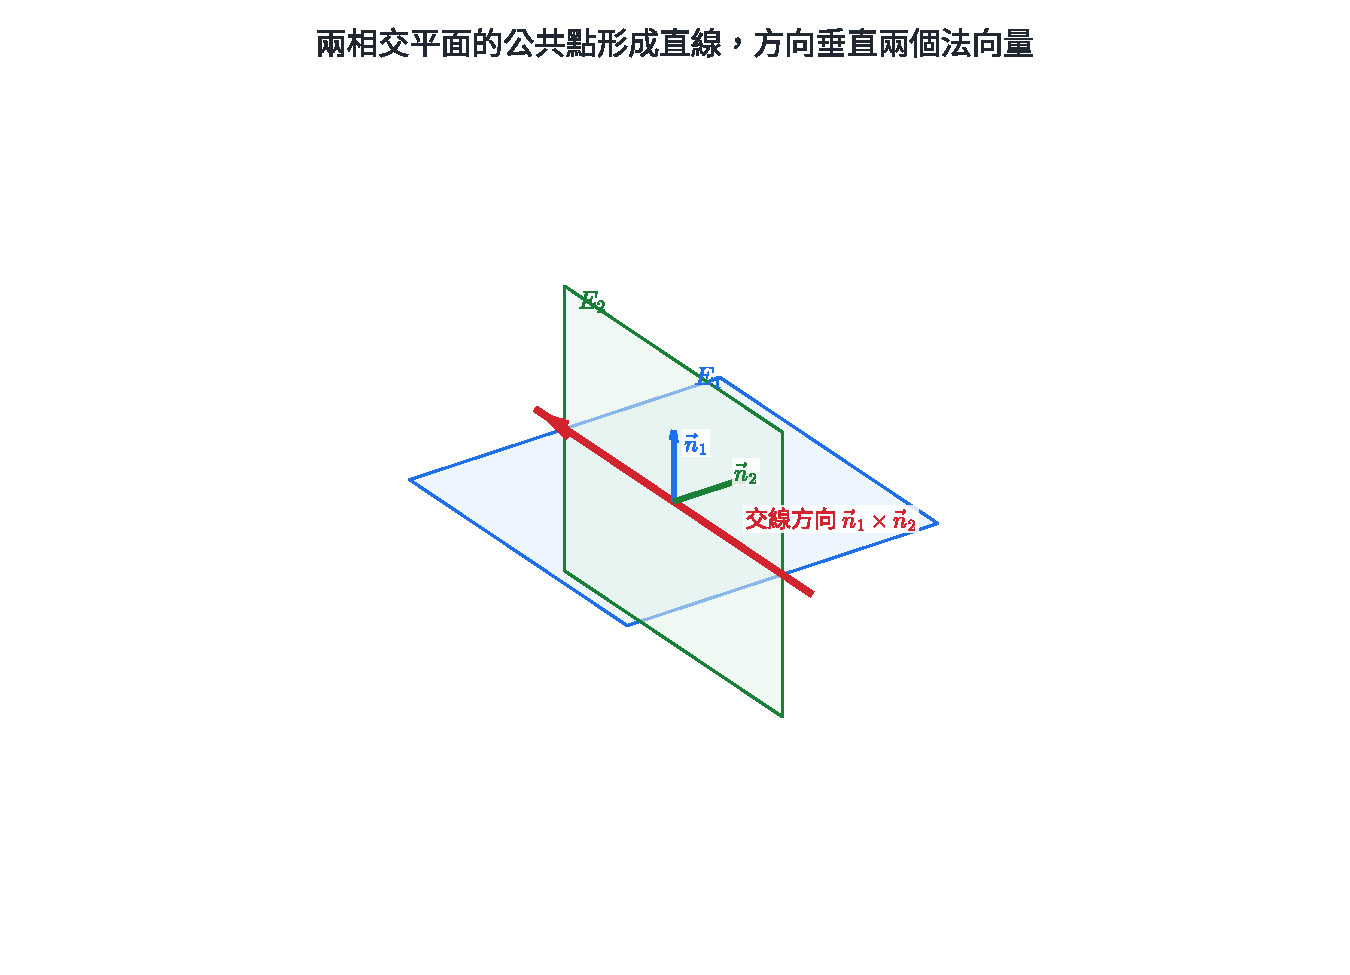
\includegraphics[width=0.82\linewidth,height=\textheight,keepaspectratio,alt={圖 7｜兩平面交線的方向垂直兩個法向量，可由外積取得。}]{assets/數A4-2-兩面交線.pdf}
\caption{圖 7｜兩平面交線的方向垂直兩個法向量，可由外積取得。}
\end{figure}

兩個平面方程式直接聯立的表示稱為直線的兩面式。它適合描述交集；參數式則適合找點、判斷交會與建立運動模型。

\subsection{參數式同時記錄路徑與位置狀態}\label{ux53c3ux6578ux5f0fux540cux6642ux8a18ux9304ux8defux5f91ux8207ux4f4dux7f6eux72c0ux614b}

一般式回答「點是否在幾何物件上」；參數式進一步回答「沿路徑走了多少」。無人機航線 \(X(t)=A+t\vec d\) 中，若 \(t\) 與時間成比例，就能直接預測各時刻位置；電腦繪圖的射線追蹤也沿 \(A+t\vec d\) 尋找光線與物體表面的第一個交點。

\begin{HandoutWorkedExample}

\subsection{完整示範｜由兩點寫出參數式與比例式}\label{ux5b8cux6574ux793aux7bc4ux7531ux5169ux9edeux5bebux51faux53c3ux6578ux5f0fux8207ux6bd4ux4f8bux5f0f}

直線通過

\[
P=(1,-2,3),\qquad Q=(5,0,-1).
\]

方向向量

\[
\overrightarrow{PQ}=(4,2,-4)=2(2,1,-2).
\]

取較簡單的 \(\vec d=(2,1,-2)\)，參數式為

\[
\boxed{
\begin{cases}
x=1+2t,\\
y=-2+t,\\
z=3-2t.
\end{cases}}
\]

比例式為

\[
\boxed{
\frac{x-1}{2}=y+2=\frac{z-3}{-2}
}.
\]

點 \(Q\) 對應 \(t=2\)，代入三式分別得到 \((5,0,-1)\)。

\end{HandoutWorkedExample}

\begin{HandoutWorkedExample}

\subsection{完整示範｜方向分量為零的比例式}\label{ux5b8cux6574ux793aux7bc4ux65b9ux5411ux5206ux91cfux70baux96f6ux7684ux6bd4ux4f8bux5f0f}

直線通過 \(A=(2,3,-1)\)，方向向量為 \((2,0,-3)\)。

參數式：

\[
\begin{cases}
x=2+2t,\\
y=3,\\
z=-1-3t.
\end{cases}
\]

比例式：

\[
\boxed{
\frac{x-2}{2}=\frac{z+1}{-3},
\qquad y=3
}.
\]

\(y\) 坐標固定為 \(3\)，表示直線平行 \(xz\) 平面。

\end{HandoutWorkedExample}

\begin{HandoutWorkedExample}

\subsection{完整示範｜把兩面式化為參數式}\label{ux5b8cux6574ux793aux7bc4ux628aux5169ux9762ux5f0fux5316ux70baux53c3ux6578ux5f0f}

兩平面

\[
E_1:x+y+z=3,
\qquad
E_2:x-y+z=1
\]

交於直線 \(L\)。法向量為

\[
\vec n_1=(1,1,1),
\qquad
\vec n_2=(1,-1,1).
\]

外積

\[
\vec n_1\times\vec n_2=(2,0,-2)=2(1,0,-1),
\]

所以方向可取 \((1,0,-1)\)。

聯立兩平面，兩式相減得 \(2y=2\)，所以 \(y=1\)；再得 \(x+z=2\)。取 \(z=0\)，可得公共點 \(A=(2,1,0)\)。因此

\[
\boxed{
L:(x,y,z)=(2,1,0)+t(1,0,-1)
}.
\]

代入兩個平面方程式都分別得到 \(3\) 與 \(1\)，且與 \(t\) 無關。

\end{HandoutWorkedExample}

\begin{HandoutSelfCheck}

\subsection{節末練習｜直線方程式}\label{ux7bc0ux672bux7df4ux7fd2ux76f4ux7ddaux65b9ux7a0bux5f0f}

\begin{enumerate}
\def\labelenumi{\arabic{enumi}.}
\tightlist
\item
  寫出通過 \(A=(1,2,-1)\)、方向向量 \((3,-2,4)\) 的參數式與比例式。
\item
  求通過 \(P=(-1,0,2)\)、\(Q=(3,6,0)\) 的直線參數式。
\item
  把 \(x=2+t\)、\(y=-1+3t\)、\(z=4\) 寫成比例式。
\item
  判斷點 \(R=(5,0,-5)\) 是否在直線 \((x,y,z)=(1,2,1)+t(2,-1,-3)\) 上。
\item
  求平面 \(x+y-z=1\) 與 \(2x-y+z=4\) 的交線參數式。
\item
  寫出線段 \(A=(0,1,2)\) 到 \(B=(4,-1,6)\) 的參數表示，並給出對應線段的參數範圍。
\end{enumerate}

\textbf{解答}

\begin{enumerate}
\def\labelenumi{\arabic{enumi}.}
\tightlist
\item
  參數式 \((x,y,z)=(1,2,-1)+t(3,-2,4)\)；比例式 \(\dfrac{x-1}{3}=\dfrac{y-2}{-2}=\dfrac{z+1}{4}\)。
\item
  \(Q-P=(4,6,-2)=2(2,3,-1)\)，可寫成 \((x,y,z)=(-1,0,2)+t(2,3,-1)\)。
\item
  \(z=4\) 固定，其餘兩式消去 \(t\)：\(\boxed{x-2=(y+1)/3,\ z=4}\)。
\item
  由 \(x\) 得 \(t=2\)，由 \(y\) 也得 \(t=2\)，但此時 \(z=1-6=-5\)，一致，所以 \(R\) 在直線上。
\item
  法向量 \((1,1,-1)\)、\((2,-1,1)\) 的外積為 \((0,-3,-3)\)，方向可取 \((0,1,1)\)。令 \(z=0\)，聯立得 \(x=5/3,y=-2/3\)，所以 \(L=(5/3,-2/3,0)+t(0,1,1)\)。
\item
  \(X=A+t(B-A)=(0,1,2)+t(4,-2,4)\)，線段對應 \(\boxed{0\le t\le1}\)。
\end{enumerate}

\end{HandoutSelfCheck}

\section{4. 直線與平面的關係、投影與夾角}\label{ux76f4ux7ddaux8207ux5e73ux9762ux7684ux95dcux4fc2ux6295ux5f71ux8207ux593eux89d2}

\subsection{4.1 用方向向量與代入結果判斷交集}\label{ux7528ux65b9ux5411ux5411ux91cfux8207ux4ee3ux5165ux7d50ux679cux5224ux65b7ux4ea4ux96c6}

設直線

\[
L:X=A+t\vec d
\]

與平面

\[
E:\vec n\cdot X+d_0=0.
\]

把直線代入平面：

\[
\vec n\cdot(A+t\vec d)+d_0
=F(A)+t(\vec n\cdot\vec d)=0.
\]

參數方程的解數量直接對應幾何交集：

{\def\LTcaptype{none} % do not increment counter
\begin{longtable}[]{@{}lrl@{}}
\toprule\noalign{}
條件 & 參數解 & 幾何關係 \\
\midrule\noalign{}
\endhead
\bottomrule\noalign{}
\endlastfoot
\(\vec n\cdot\vec d\ne0\) & 唯一解 & 相交於一點 \\
\(\vec n\cdot\vec d=0\) 且 \(F(A)\ne0\) & 無解 & 直線平行平面 \\
\(\vec n\cdot\vec d=0\) 且 \(F(A)=0\) & 所有 \(t\) & 直線在平面內 \\
\end{longtable}
}

\begin{figure}
\centering
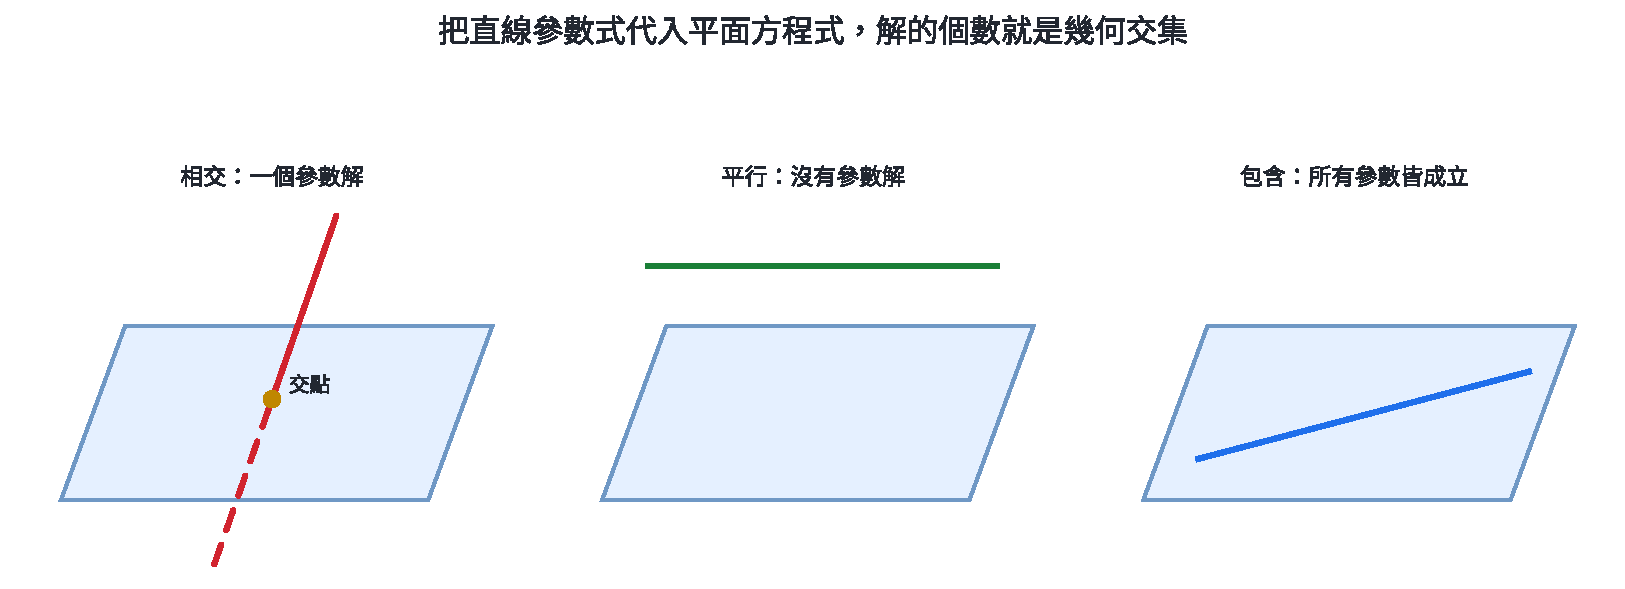
\includegraphics[width=0.96\linewidth,height=\textheight,keepaspectratio,alt={圖 8｜代入後一元一次方程的解數，分別對應相交、平行與包含。}]{assets/數A4-2-直線與平面關係.pdf}
\caption{圖 8｜代入後一元一次方程的解數，分別對應相交、平行與包含。}
\end{figure}

\subsection{4.2 包含直線的平面}\label{ux5305ux542bux76f4ux7ddaux7684ux5e73ux9762}

平面若包含直線 \(L\)，平面的法向量必須垂直 \(L\) 的方向向量。要決定唯一平面，還需另一個獨立的平面內方向。

若平面包含直線 \(L:X=A+t\vec d\)，並通過線外一點 \(P\)，可取

\[
\overrightarrow{AP}=P-A
\]

作為第二個平面內方向，因此法向量可取

\[
\boxed{\vec n=\vec d\times\overrightarrow{AP}}.
\]

兩條相交直線或兩條平行直線也能決定唯一平面；分別取兩方向向量，或取一個方向向量與兩線間位移，再作外積。

\subsection{4.3 點在平面上的投影與對稱}\label{ux9edeux5728ux5e73ux9762ux4e0aux7684ux6295ux5f71ux8207ux5c0dux7a31}

投影公式沿用上一節：

\[
Q=P-\frac{F(P)}{|\vec n|^2}\vec n.
\]

它也可以用聯立法理解：過 \(P\) 作方向為 \(\vec n\) 的直線，與平面的唯一交點就是 \(Q\)。對稱點 \(P'=2Q-P\)。

\begin{figure}
\centering
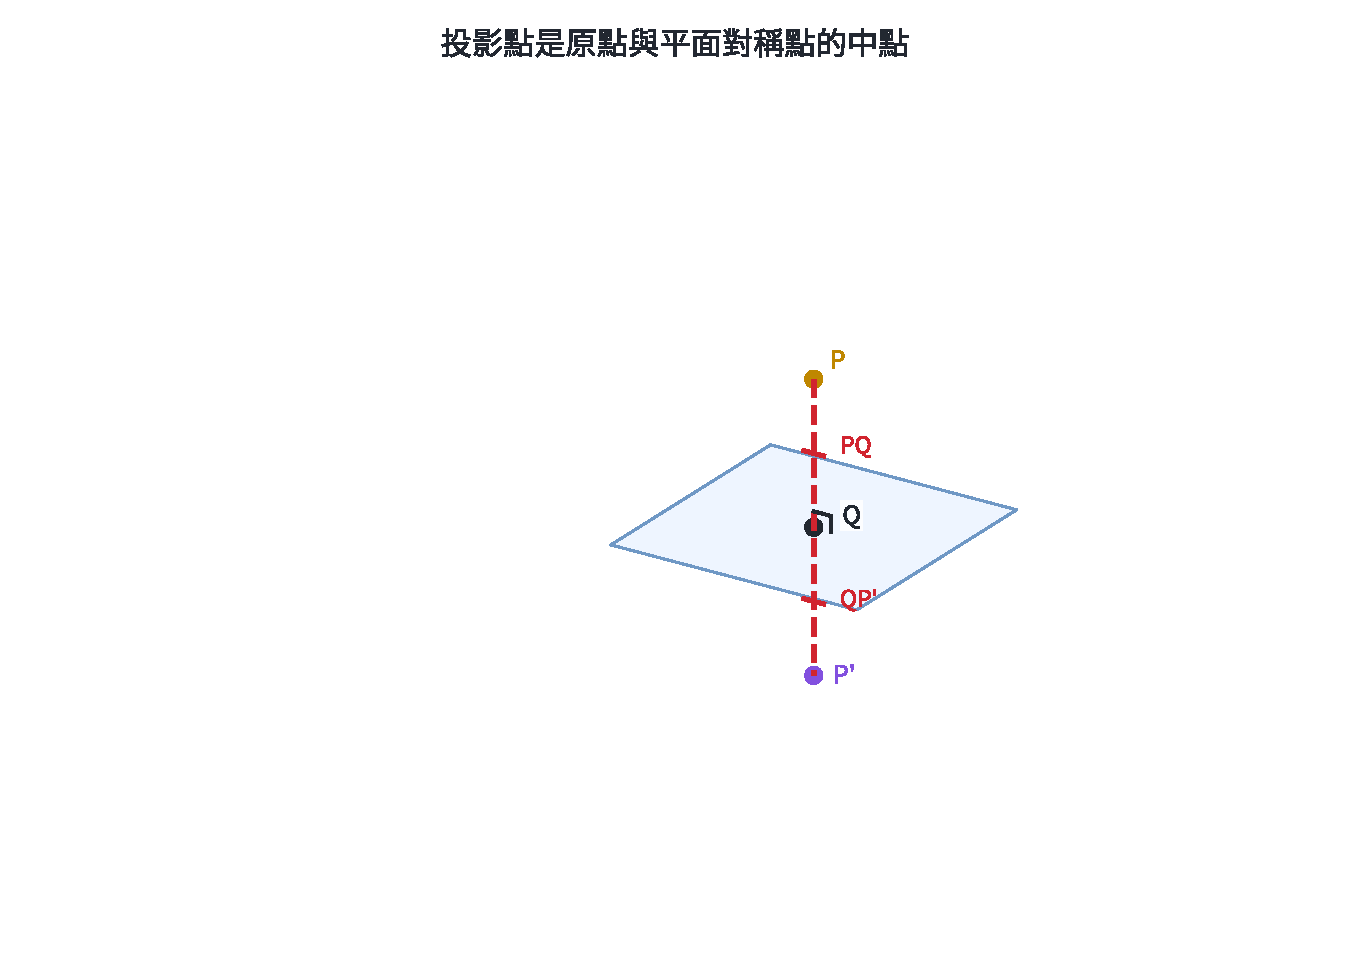
\includegraphics[width=0.82\linewidth,height=\textheight,keepaspectratio,alt={圖 9｜投影點 Q 位於平面上，且 PQ 沿法向量；對稱點使 Q 成為 PP\textquotesingle{} 中點。}]{assets/數A4-2-平面投影與對稱.pdf}
\caption{圖 9｜投影點 \(Q\) 位於平面上，且 \(PQ\) 沿法向量；對稱點使 \(Q\) 成為 \(PP'\) 中點。}
\end{figure}

\subsection{4.4 直線與平面的夾角}\label{ux76f4ux7ddaux8207ux5e73ux9762ux7684ux593eux89d2}

設直線方向向量 \(\vec d\) 與平面法向量 \(\vec n\) 的銳夾角為 \(\alpha\)，直線與平面的夾角為 \(\theta\)，則

\[
\alpha+\theta=90^\circ.
\]

因此

\[
\boxed{
\sin\theta
=\frac{|\vec d\cdot\vec n|}{|\vec d|\,|\vec n|}
},
\qquad0^\circ\le\theta\le90^\circ.
\]

\begin{figure}
\centering
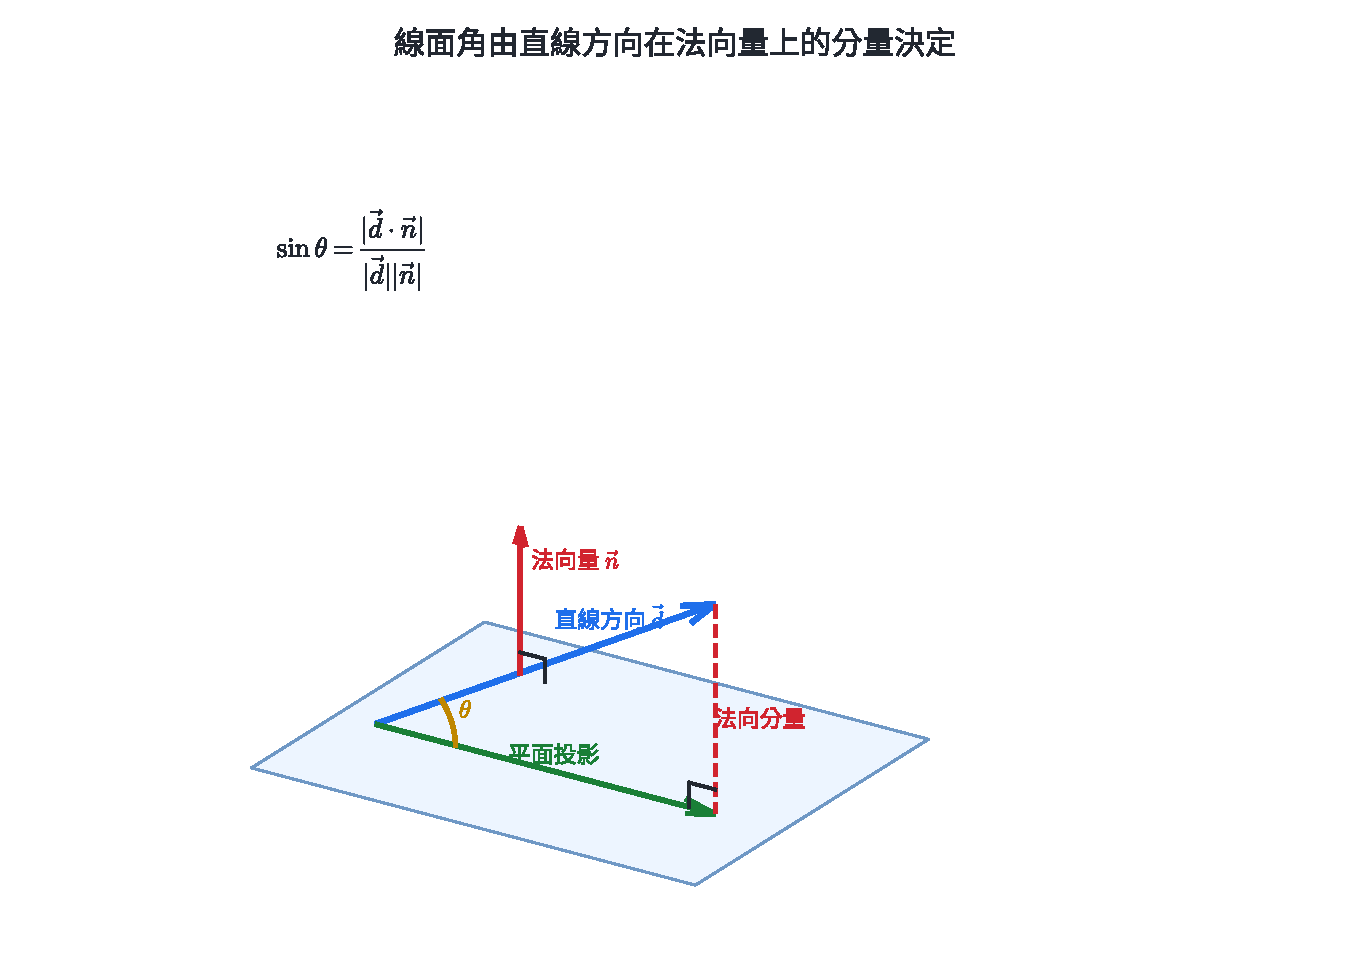
\includegraphics[width=0.84\linewidth,height=\textheight,keepaspectratio,alt={圖 10｜直線在法向量上的投影決定離開平面的程度，因此線面角使用正弦。}]{assets/數A4-2-直線與平面夾角.pdf}
\caption{圖 10｜直線在法向量上的投影決定離開平面的程度，因此線面角使用正弦。}
\end{figure}

\(\vec d\cdot\vec n=0\) 時，直線方向完全留在平面方向中，線面角為 \(0^\circ\)；\(\vec d\parallel\vec n\) 時，線面角為 \(90^\circ\)。

\begin{HandoutWorkedExample}

\subsection{完整示範｜判斷平行並核對位置}\label{ux5b8cux6574ux793aux7bc4ux5224ux65b7ux5e73ux884cux4e26ux6838ux5c0dux4f4dux7f6e}

直線

\[
L:(x,y,z)=(1,0,2)+t(2,1,-1)
\]

與平面

\[
E:x-y+z=4.
\]

方向向量 \(\vec d=(2,1,-1)\)，法向量 \(\vec n=(1,-1,1)\)。先算

\[
\vec n\cdot\vec d=2-1-1=0,
\]

所以直線方向平行平面。再代入基準點 \(A=(1,0,2)\)：

\[
1-0+2=3\ne4.
\]

因此直線不在平面上，而是

\[
\boxed{L\parallel E}.
\]

\end{HandoutWorkedExample}

\begin{HandoutWorkedExample}

\subsection{完整示範｜求直線與平面的交點}\label{ux5b8cux6574ux793aux7bc4ux6c42ux76f4ux7ddaux8207ux5e73ux9762ux7684ux4ea4ux9ede}

同一直線

\[
L:(x,y,z)=(1,0,2)+t(2,1,-1)
\]

改與平面 \(E:x+y+z=4\) 相交。代入：

\[
(1+2t)+t+(2-t)=4,
\]

\[
3+2t=4,
\qquad t=\frac12.
\]

交點為

\[
\boxed{
I=\left(2,\frac12,\frac32\right)
}.
\]

代回平面得 \(2+1/2+3/2=4\)。

\end{HandoutWorkedExample}

\begin{HandoutWorkedExample}

\subsection{完整示範｜求包含直線與線外一點的平面}\label{ux5b8cux6574ux793aux7bc4ux6c42ux5305ux542bux76f4ux7ddaux8207ux7ddaux5916ux4e00ux9edeux7684ux5e73ux9762}

平面包含直線

\[
L:(x,y,z)=(1,0,0)+t(1,1,0)
\]

並通過 \(P=(0,1,1)\)。直線上取 \(A=(1,0,0)\)，則

\[
\vec d=(1,1,0),
\qquad
\overrightarrow{AP}=(-1,1,1).
\]

法向量可取

\[
\vec n=\vec d\times\overrightarrow{AP}
=(1,-1,2).
\]

代入點 \(A\)：

\[
(x-1)-y+2z=0.
\]

所以

\[
\boxed{x-y+2z-1=0}.
\]

把直線參數代入得 \((1+t)-t-1=0\)，對所有 \(t\) 成立；代入 \(P\) 也得到 \(0\)。

\end{HandoutWorkedExample}

\begin{HandoutWorkedExample}

\subsection{完整示範｜平面投影與對稱點}\label{ux5b8cux6574ux793aux7bc4ux5e73ux9762ux6295ux5f71ux8207ux5c0dux7a31ux9ede}

點 \(P=(3,-1,4)\)，平面

\[
E:2x-y+2z-3=0.
\]

\(\vec n=(2,-1,2)\)，\(|\vec n|^2=9\)，且

\[
F(P)=6+1+8-3=12.
\]

投影點

\[
Q=P-\frac{12}{9}(2,-1,2)
=\boxed{\left(\frac13,\frac13,\frac43\right)}.
\]

對稱點

\[
P'=2Q-P
=\boxed{\left(-\frac73,\frac53,-\frac43\right)}.
\]

核對 \(Q\) 在平面上：\(2/3-1/3+8/3-3=0\)。

\end{HandoutWorkedExample}

\begin{HandoutWorkedExample}

\subsection{完整示範｜求直線與平面的夾角}\label{ux5b8cux6574ux793aux7bc4ux6c42ux76f4ux7ddaux8207ux5e73ux9762ux7684ux593eux89d2}

直線方向向量為 \(\vec d=(2,-1,2)\)，平面法向量為 \(\vec n=(1,2,2)\)。兩向量長皆為 \(3\)，且

\[
\vec d\cdot\vec n=2-2+4=4.
\]

若線面角為 \(\theta\)，

\[
\sin\theta=\frac49,
\]

\[
\boxed{\theta=\sin^{-1}\!\left(\frac49\right)\approx26.4^\circ}.
\]

\end{HandoutWorkedExample}

\begin{HandoutSelfCheck}

\subsection{節末練習｜直線與平面}\label{ux7bc0ux672bux7df4ux7fd2ux76f4ux7ddaux8207ux5e73ux9762}

\begin{enumerate}
\def\labelenumi{\arabic{enumi}.}
\tightlist
\item
  判斷直線 \((x,y,z)=(1,2,0)+t(1,-1,2)\) 與平面 \(x+y=3\) 的關係。
\item
  求直線 \((x,y,z)=(0,1,2)+t(2,-1,1)\) 與平面 \(x+2y-z=1\) 的交點。
\item
  求包含直線 \((x,y,z)=(1,0,1)+t(1,2,0)\) 且通過 \(P=(0,1,3)\) 的平面。
\item
  求點 \(P=(2,-1,3)\) 在平面 \(x+2y+2z-5=0\) 上的投影點。
\item
  求第 4 題中 \(P\) 關於該平面的對稱點。
\item
  求方向向量 \((1,2,2)\) 的直線與平面 \(2x-y+2z=4\) 的銳夾角。
\end{enumerate}

\textbf{解答}

\begin{enumerate}
\def\labelenumi{\arabic{enumi}.}
\tightlist
\item
  法向量 \((1,1,0)\) 與方向向量內積為 \(0\)；基準點滿足 \(1+2=3\)，所以整條直線在平面內。
\item
  代入得 \(2t+2(1-t)-(2+t)=1\)，即 \(-t=1\)，所以 \(t=-1\)，交點為 \(\boxed{(-2,2,1)}\)。
\item
  取 \(A=(1,0,1)\)、\(\vec d=(1,2,0)\)、\(\overrightarrow{AP}=(-1,1,2)\)。外積為 \((4,-2,3)\)，所以平面為 \(\boxed{4x-2y+3z-7=0}\)。
\item
  \(F(P)=2-2+6-5=1\)，\(|\vec n|^2=9\)，故 \(Q=P-\tfrac19(1,2,2)=\boxed{(17/9,-11/9,25/9)}\)。
\item
  \(P'=2Q-P=\boxed{(16/9,-13/9,23/9)}\)。
\item
  \(\vec d=(1,2,2)\)、\(\vec n=(2,-1,2)\)，內積為 \(4\)，長度皆 \(3\)，所以 \(\theta=\sin^{-1}(4/9)\approx26.4^\circ\)。
\end{enumerate}

\end{HandoutSelfCheck}

\section{5. 兩直線的位置關係與夾角}\label{ux5169ux76f4ux7ddaux7684ux4f4dux7f6eux95dcux4fc2ux8207ux593eux89d2}

\subsection{5.1 方向向量先分流}\label{ux65b9ux5411ux5411ux91cfux5148ux5206ux6d41}

設

\[
L_1:X=A+t\vec d_1,
\qquad
L_2:X=B+s\vec d_2.
\]

先判斷 \(\vec d_1,\vec d_2\) 是否平行：

\begin{itemize}
\item
  若方向平行，再檢查 \(B-A\) 是否也平行該方向。是則兩線重合；否則兩線平行且不同。
\item
  若方向不平行，聯立

  \[
  A+t\vec d_1=B+s\vec d_2.
  \]

  三個分量有共同的 \((t,s)\) 解時，兩線相交；無共同解時，兩線歪斜。
\end{itemize}

\begin{figure}
\centering
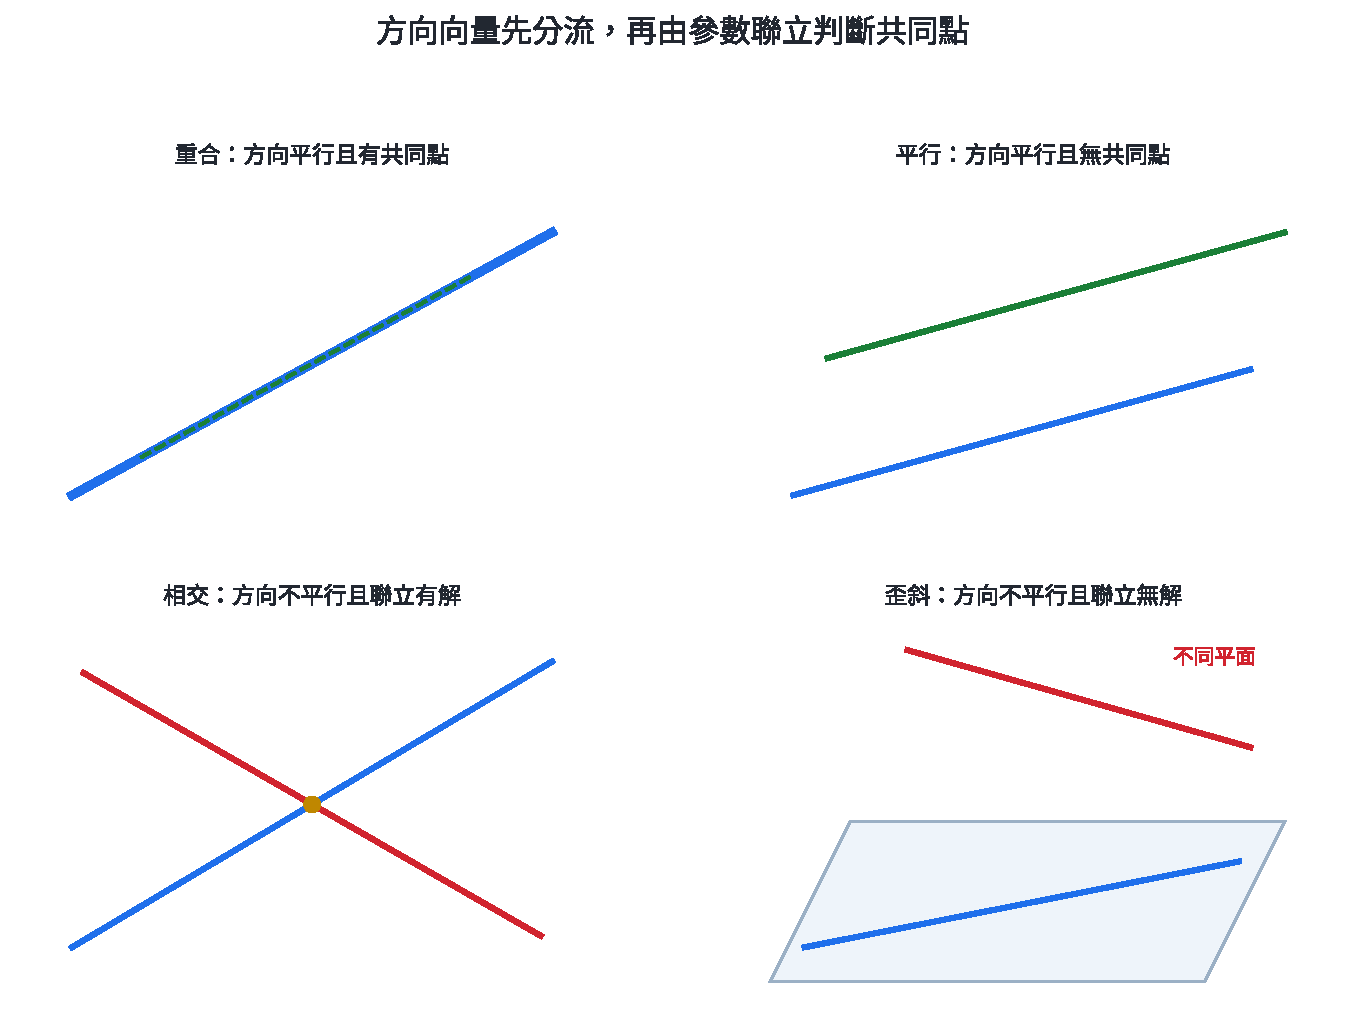
\includegraphics[width=0.94\linewidth,height=\textheight,keepaspectratio,alt={圖 11｜方向向量先區分平行類與非平行類，再由共同點區分重合、平行、相交與歪斜。}]{assets/數A4-2-兩直線判別.pdf}
\caption{圖 11｜方向向量先區分平行類與非平行類，再由共同點區分重合、平行、相交與歪斜。}
\end{figure}

歪斜線是空間特有的關係：兩線方向不平行，卻因位於不同平面而沒有交點。

也可用三重積檢查共面。若 \(\vec d_1,\vec d_2\) 不平行，則

\[
\boxed{
L_1,L_2\text{ 共面}
\iff
(B-A)\cdot(\vec d_1\times\vec d_2)=0
}.
\]

共面且方向不平行就會相交；三重積非零則為歪斜。

\subsection{5.2 兩直線的銳夾角}\label{ux5169ux76f4ux7ddaux7684ux92b3ux593eux89d2}

兩直線的夾角由方向向量決定。取銳角或直角 \(\theta\)：

\[
\boxed{
\cos\theta=
\frac{|\vec d_1\cdot\vec d_2|}
{|\vec d_1|\,|\vec d_2|}
},
\qquad0^\circ\le\theta\le90^\circ.
\]

即使兩線歪斜，仍可把其中一條平移到與另一條相交，再以方向向量定義夾角。

\begin{HandoutWorkedExample}

\subsection{完整示範｜聯立參數找交點}\label{ux5b8cux6574ux793aux7bc4ux806fux7acbux53c3ux6578ux627eux4ea4ux9ede}

\[
L_1:(x,y,z)=t(1,1,1),
\]

\[
L_2:(x,y,z)=(1,3,1)+s(1,-1,1).
\]

方向向量不平行。聯立三個分量：

\[
\begin{cases}
t=1+s,\\
t=3-s,\\
t=1+s.
\end{cases}
\]

前兩式給 \(2s=2\)，所以 \(s=1\)、\(t=2\)；第三式也成立。因此兩線交於

\[
\boxed{I=(2,2,2)}.
\]

\end{HandoutWorkedExample}

\begin{HandoutWorkedExample}

\subsection{完整示範｜方向平行時區分重合與平行}\label{ux5b8cux6574ux793aux7bc4ux65b9ux5411ux5e73ux884cux6642ux5340ux5206ux91cdux5408ux8207ux5e73ux884c}

\[
L_1:X=(1,0,2)+t(2,-1,1).
\]

先看

\[
L_2:X=(5,-2,4)+s(-4,2,-2).
\]

\(L_2\) 的方向是 \(L_1\) 方向的 \(-2\) 倍；而

\[
(5,-2,4)-(1,0,2)=(4,-2,2)=2(2,-1,1),
\]

所以 \(L_2\) 的基準點也在 \(L_1\) 上，兩線重合。

若把 \(L_2\) 的基準點改成 \((5,-2,5)\)，兩方向仍平行，但位移 \((4,-2,3)\) 不是 \((2,-1,1)\) 的倍數，因此兩線平行且不同。

\end{HandoutWorkedExample}

\begin{HandoutWorkedExample}

\subsection{完整示範｜以三重積判斷歪斜}\label{ux5b8cux6574ux793aux7bc4ux4ee5ux4e09ux91cdux7a4dux5224ux65b7ux6b6aux659c}

\[
L_1:X=(0,0,0)+t(1,0,1),
\]

\[
L_2:X=(0,1,0)+s(0,1,1).
\]

方向向量不平行。取

\[
B-A=(0,1,0),
\]

\[
\vec d_1\times\vec d_2
=(1,0,1)\times(0,1,1)
=(-1,-1,1).
\]

三重積

\[
(0,1,0)\cdot(-1,-1,1)=-1\ne0.
\]

所以兩線不共面，結論為

\[
\boxed{L_1,L_2\text{ 歪斜}}.
\]

\end{HandoutWorkedExample}

\begin{HandoutWorkedExample}

\subsection{完整示範｜兩直線的夾角}\label{ux5b8cux6574ux793aux7bc4ux5169ux76f4ux7ddaux7684ux593eux89d2}

方向向量

\[
\vec d_1=(1,2,2),
\qquad
\vec d_2=(2,1,-2).
\]

內積為

\[
\vec d_1\cdot\vec d_2=2+2-4=0.
\]

所以兩直線夾角為

\[
\boxed{90^\circ}.
\]

這個結論只由方向決定，適用於相交線或歪斜線。

\end{HandoutWorkedExample}

\begin{HandoutSelfCheck}

\subsection{節末練習｜兩直線關係}\label{ux7bc0ux672bux7df4ux7fd2ux5169ux76f4ux7ddaux95dcux4fc2}

\begin{enumerate}
\def\labelenumi{\arabic{enumi}.}
\tightlist
\item
  判斷 \(L_1:X=(1,0,1)+t(2,-1,3)\) 與 \(L_2:X=(5,-2,7)+s(-4,2,-6)\) 的關係。
\item
  判斷 \(L_1:X=t(1,2,1)\) 與 \(L_2:X=(1,0,2)+s(1,-1,0)\) 是否相交；若相交，求交點。
\item
  用三重積判斷 \(L_1:X=t(1,0,1)\) 與 \(L_2:X=(0,2,0)+s(1,1,0)\) 是否歪斜。
\item
  求方向向量 \((1,1,0)\) 與 \((1,0,1)\) 所代表兩直線的銳夾角。
\item
  已知兩直線方向向量為 \((1,k,1)\) 與 \((2,-1,0)\)，且兩線垂直，求 \(k\)。
\item
  寫出通過原點且與直線 \((x,y,z)=(1,2,3)+t(2,-1,2)\) 平行的直線。
\end{enumerate}

\textbf{解答}

\begin{enumerate}
\def\labelenumi{\arabic{enumi}.}
\tightlist
\item
  方向向量成 \(-2\) 倍，且基準點位移 \((4,-2,6)=2(2,-1,3)\)，所以兩線重合。
\item
  聯立 \((t,2t,t)=(1+s,-s,2)\)。由第三式 \(t=2\)，第二式給 \(s=-4\)，但第一式變成 \(2=-3\)，矛盾；方向不平行且無交點，所以歪斜。
\item
  \(B-A=(0,2,0)\)，\(\vec d_1\times\vec d_2=(1,0,1)\times(1,1,0)=(-1,1,1)\)。三重積為 \(2\ne0\)，所以歪斜。
\item
  內積為 \(1\)，長度皆 \(\sqrt2\)，所以 \(\cos\theta=1/2\)，\(\boxed{\theta=60^\circ}\)。
\item
  內積 \(2-k=0\)，所以 \(\boxed{k=2}\)。
\item
  可寫成 \(\boxed{(x,y,z)=t(2,-1,2)}\)。
\end{enumerate}

\end{HandoutSelfCheck}

\section{6. 與直線相關的最短距離}\label{ux8207ux76f4ux7ddaux76f8ux95dcux7684ux6700ux77edux8dddux96e2}

\subsection{6.1 點到直線}\label{ux9edeux5230ux76f4ux7dda}

直線 \(L:X=A+t\vec d\)，點 \(P\)。垂足 \(H=A+t_0\vec d\) 要滿足

\[
\overrightarrow{HP}\cdot\vec d=0.
\]

也就是

\[
(P-A-t_0\vec d)\cdot\vec d=0,
\]

所以

\[
\boxed{
t_0=\frac{\overrightarrow{AP}\cdot\vec d}{|\vec d|^2}
},
\]

\[
\boxed{
H=A+t_0\vec d,
\qquad
d(P,L)=|P-H|
}.
\]

\begin{figure}
\centering
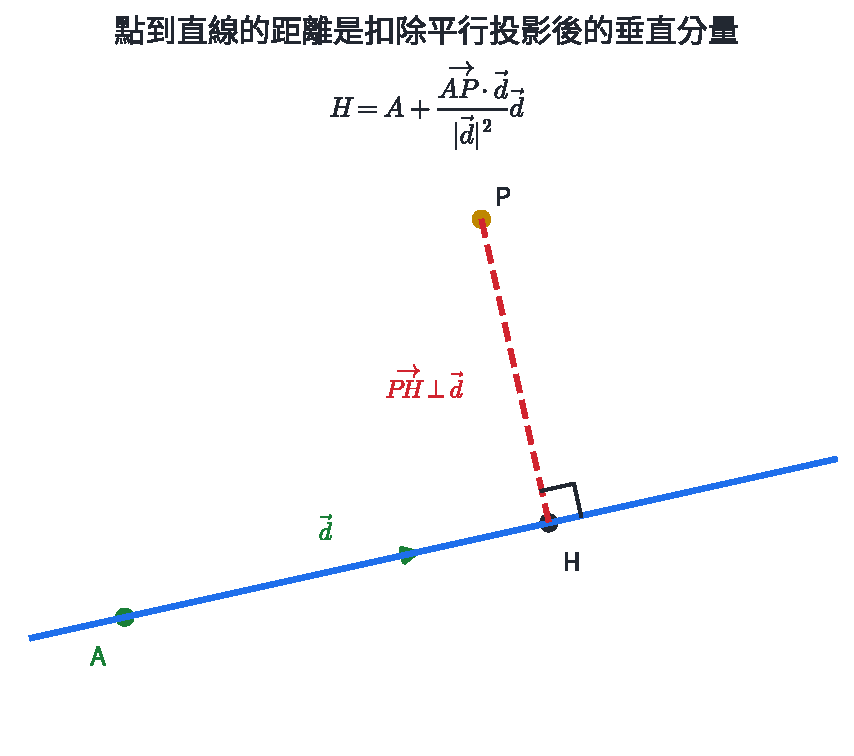
\includegraphics[width=0.86\linewidth,height=\textheight,keepaspectratio,alt={圖 12｜垂足把點到直線的位移分成平行投影與垂直分量；垂直分量最短。}]{assets/數A4-2-點到直線距離.pdf}
\caption{圖 12｜垂足把點到直線的位移分成平行投影與垂直分量；垂直分量最短。}
\end{figure}

以外積的面積觀點，也可寫成

\[
\boxed{
d(P,L)=
\frac{|\overrightarrow{AP}\times\vec d|}{|\vec d|}
}.
\]

分子是以 \(|\vec d|\) 為底、點線距離為高的平行四邊形面積。

\subsection{6.2 兩平行線}\label{ux5169ux5e73ux884cux7dda}

兩平行線的距離固定。任取 \(L_1\) 上一點 \(A\)，求它到 \(L_2\) 的點線距離即可：\(\boxed{d(L_1,L_2)=\frac{|\overrightarrow{BA}\times\vec d|}{|\vec d|}}\)，其中 \(B\) 是 \(L_2\) 上任一點，\(\vec d\) 是共同方向。

\subsection{6.3 兩歪斜線}\label{ux5169ux6b6aux659cux7dda}

設

\[
L_1:X=A+t\vec d_1,
\qquad
L_2:X=B+s\vec d_2,
\]

而且兩線歪斜。最短連線方向同時垂直 \(\vec d_1,\vec d_2\)，所以平行

\[
\vec n=\vec d_1\times\vec d_2.
\]

把 \(\overrightarrow{AB}\) 沿 \(\vec n\) 投影，就得到距離：

\[
\boxed{
d(L_1,L_2)=
\frac{|\overrightarrow{AB}\cdot(\vec d_1\times\vec d_2)|}
{|\vec d_1\times\vec d_2|}
}.
\]

\begin{figure}
\centering
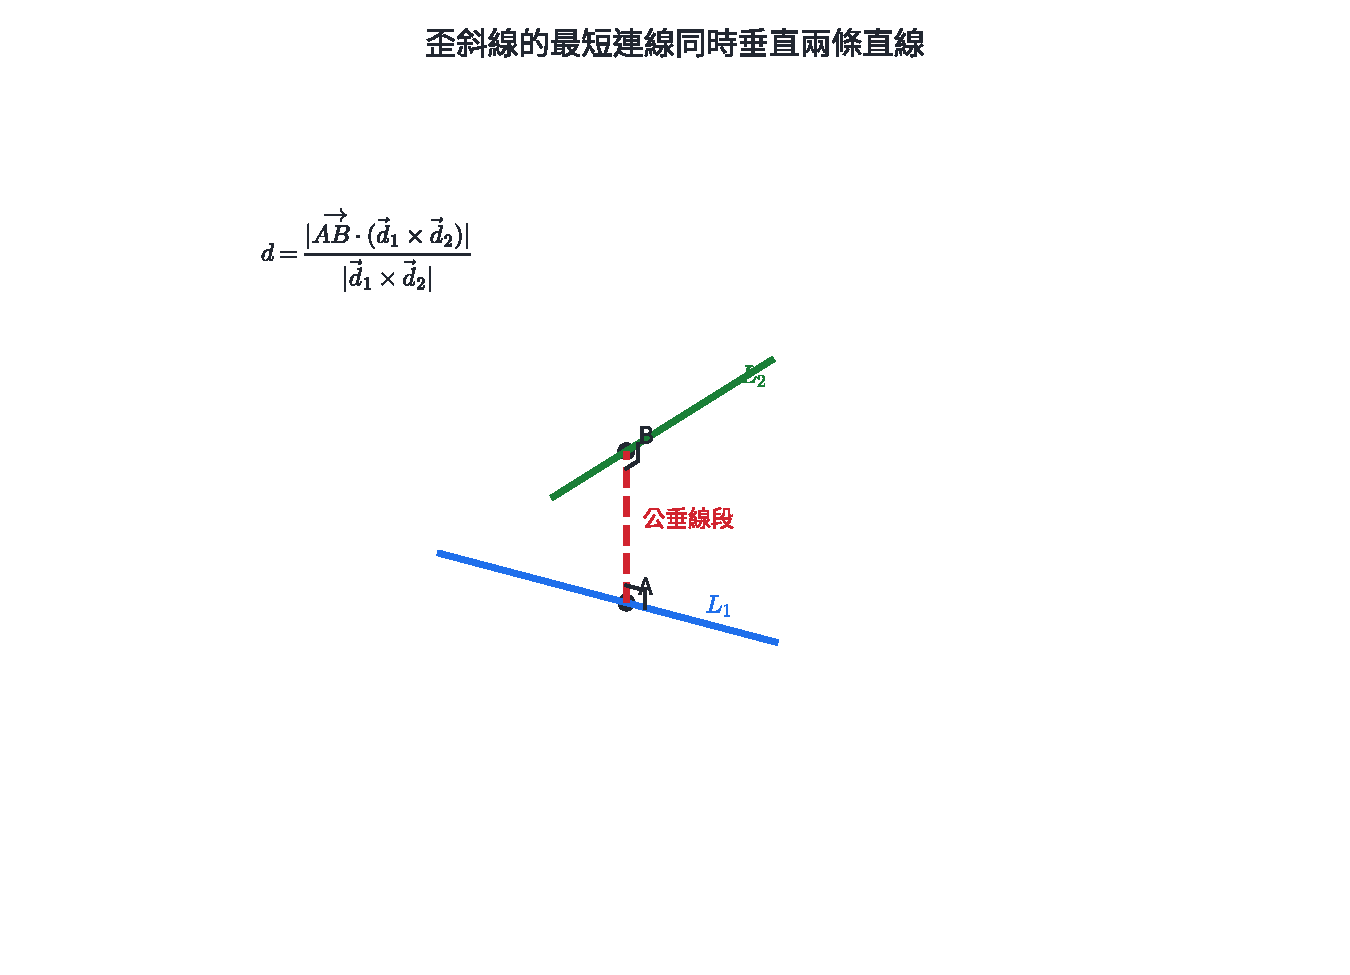
\includegraphics[width=0.84\linewidth,height=\textheight,keepaspectratio,alt={圖 13｜歪斜線的公垂線段同時垂直兩個方向；其長度就是兩線最短距離。}]{assets/數A4-2-歪斜線距離.pdf}
\caption{圖 13｜歪斜線的公垂線段同時垂直兩個方向；其長度就是兩線最短距離。}
\end{figure}

這個公式也可由體積理解。分子的絕對值是 \(\overrightarrow{AB},\vec d_1,\vec d_2\) 張成的平行六面體體積；底面積為 \(|\vec d_1\times\vec d_2|\)，體積除以底面積就得到高。

若要找公垂線的兩個端點，令

\[
P=A+t\vec d_1,
\qquad
Q=B+s\vec d_2,
\]

並解

\[
\overrightarrow{PQ}\cdot\vec d_1=0,
\qquad
\overrightarrow{PQ}\cdot\vec d_2=0.
\]

兩個一次方程可求出 \(t,s\)。

\subsection{最短距離來自「可移動方向全部被消去」}\label{ux6700ux77edux8dddux96e2ux4f86ux81eaux53efux79fbux52d5ux65b9ux5411ux5168ux90e8ux88abux6d88ux53bb}

從點連到直線時，沿直線方向的位移仍可藉由滑動垂足改變；最短位置會讓剩餘連線完全垂直直線。兩條歪斜線各有一個可移動方向，最短連線便要同時垂直兩者。

機器手臂避障、管線間隙檢查與道路立體交叉的淨距，都可化成點、平行線或歪斜線的最短距離模型。

\begin{HandoutWorkedExample}

\subsection{完整示範｜求點到直線的垂足與距離}\label{ux5b8cux6574ux793aux7bc4ux6c42ux9edeux5230ux76f4ux7ddaux7684ux5782ux8db3ux8207ux8dddux96e2}

直線

\[
L:X=(0,1,1)+t(1,2,2),
\]

點 \(P=(3,0,4)\)。令 \(A=(0,1,1)\)、\(\vec d=(1,2,2)\)，則

\[
\overrightarrow{AP}=(3,-1,3).
\]

\[
t_0=\frac{(3,-1,3)\cdot(1,2,2)}{1+4+4}
=\frac{3-2+6}{9}
=\frac79.
\]

垂足

\[
H=A+\frac79\vec d
=\boxed{\left(\frac79,\frac{23}{9},\frac{23}{9}\right)}.
\]

\[
\overrightarrow{HP}
=\left(\frac{20}{9},-\frac{23}{9},\frac{13}{9}\right),
\]

而 \(\overrightarrow{HP}\cdot\vec d=(20-46+26)/9=0\)。距離為

\[
d(P,L)
=\frac{\sqrt{400+529+169}}9
=\boxed{\frac{\sqrt{122}}3}.
\]

\end{HandoutWorkedExample}

\begin{HandoutWorkedExample}

\subsection{完整示範｜兩平行線的距離}\label{ux5b8cux6574ux793aux7bc4ux5169ux5e73ux884cux7ddaux7684ux8dddux96e2}

\[
L_1:X=t(1,2,2),
\]

\[
L_2:X=(2,0,1)+s(1,2,2).
\]

取 \(A=(0,0,0)\)、\(B=(2,0,1)\)。兩線共同方向 \(\vec d=(1,2,2)\)。計算

\[
\overrightarrow{AB}\times\vec d
=(2,0,1)\times(1,2,2)
=(-2,-3,4).
\]

所以

\[
d(L_1,L_2)
=\frac{\sqrt{4+9+16}}{3}
=\boxed{\frac{\sqrt{29}}3}.
\]

\end{HandoutWorkedExample}

\begin{HandoutWorkedExample}

\subsection{完整示範｜歪斜線距離與公垂線段}\label{ux5b8cux6574ux793aux7bc4ux6b6aux659cux7ddaux8dddux96e2ux8207ux516cux5782ux7ddaux6bb5}

\[
L_1:X=(0,0,0)+t(1,0,0),
\]

\[
L_2:X=(0,1,2)+s(0,1,0).
\]

\[
\vec d_1\times\vec d_2=(0,0,1),
\qquad
\overrightarrow{AB}=(0,1,2).
\]

因此

\[
d(L_1,L_2)
=\frac{|(0,1,2)\cdot(0,0,1)|}{1}
=\boxed2.
\]

求端點：\(P=(t,0,0)\)、\(Q=(0,1+s,2)\)，所以

\[
\overrightarrow{PQ}=(-t,1+s,2).
\]

它垂直 \((1,0,0)\) 給 \(t=0\)；垂直 \((0,1,0)\) 給 \(s=-1\)。故

\[
P=(0,0,0),\qquad Q=(0,0,2),
\]

公垂線段長為 \(2\)，與公式一致。

\end{HandoutWorkedExample}

\begin{HandoutSelfCheck}

\subsection{節末練習｜直線距離}\label{ux7bc0ux672bux7df4ux7fd2ux76f4ux7ddaux8dddux96e2}

\begin{enumerate}
\def\labelenumi{\arabic{enumi}.}
\tightlist
\item
  求點 \(P=(2,3,1)\) 到直線 \(L:X=(1,0,0)+t(1,2,2)\) 的垂足。
\item
  承第 1 題，求點線距離。
\item
  求平行線 \(L_1:X=t(2,1,2)\) 與 \(L_2:X=(1,2,0)+s(2,1,2)\) 的距離。
\item
  求歪斜線 \(L_1:X=t(1,0,0)\)、\(L_2:X=(1,2,3)+s(0,1,0)\) 的距離。
\item
  承第 4 題，求公垂線段在兩線上的端點。
\item
  說明點線距離的投影公式與外積公式得到同一個量的幾何理由。
\end{enumerate}

\textbf{解答}

\begin{enumerate}
\def\labelenumi{\arabic{enumi}.}
\tightlist
\item
  \(A=(1,0,0)\)、\(\overrightarrow{AP}=(1,3,1)\)、\(\vec d=(1,2,2)\)。\(t_0=(1+6+2)/9=1\)，所以垂足 \(H=(2,2,2)\)。
\item
  \(P-H=(0,1,-1)\)，距離為 \(\boxed{\sqrt2}\)。
\item
  取 \(A=(0,0,0)\)、\(B=(1,2,0)\)。\((1,2,0)\times(2,1,2)=(4,-2,-3)\)，所以距離為 \(\boxed{\sqrt{29}/3}\)。
\item
  方向外積為 \((0,0,1)\)，\(\overrightarrow{AB}=(1,2,3)\)，所以距離為 \(\boxed3\)。
\item
  \(P=(t,0,0)\)、\(Q=(1,2+s,3)\)，\(Q-P=(1-t,2+s,3)\)。垂直兩方向給 \(t=1\)、\(s=-2\)，端點為 \((1,0,0)\)、\((1,0,3)\)。
\item
  投影公式扣除沿直線方向的分量，剩下垂直分量長；外積公式先算以方向向量為底、垂直分量為高的平行四邊形面積，再除以底長。兩者都量同一個高。
\end{enumerate}

\end{HandoutSelfCheck}

\section{7. 核心整理}\label{ux6838ux5fc3ux6574ux7406}

\subsection{平面}\label{ux5e73ux9762}

\[
E:a(x-x_0)+b(y-y_0)+c(z-z_0)=0,
\qquad
\vec n=(a,b,c).
\]

\[
d(P,E)=\frac{|F(P)|}{|\vec n|},
\qquad
Q=P-\frac{F(P)}{|\vec n|^2}\vec n.
\]

\subsection{直線}\label{ux76f4ux7dda}

\[
L:X=A+t\vec d,
\qquad
\frac{x-x_0}{a}=\frac{y-y_0}{b}=\frac{z-z_0}{c}
\]

其中比例式只對非零方向分量使用；零分量改寫成固定坐標。

\subsection{關係與角度}\label{ux95dcux4fc2ux8207ux89d2ux5ea6}

\[
\cos\angle(E_1,E_2)
=\frac{|\vec n_1\cdot\vec n_2|}{|\vec n_1||\vec n_2|},
\]

\[
\sin\angle(L,E)
=\frac{|\vec d\cdot\vec n|}{|\vec d||\vec n|},
\]

\[
\cos\angle(L_1,L_2)
=\frac{|\vec d_1\cdot\vec d_2|}{|\vec d_1||\vec d_2|}.
\]

\subsection{直線距離}\label{ux76f4ux7ddaux8dddux96e2}

\[
d(P,L)=\frac{|\overrightarrow{AP}\times\vec d|}{|\vec d|},
\]

\[
d(L_1,L_2)_{\text{歪斜}}
=\frac{|\overrightarrow{AB}\cdot(\vec d_1\times\vec d_2)|}{|\vec d_1\times\vec d_2|}.
\]

平面用法向量描述限制；直線用方向向量描述自由移動；交集靠聯立，最短距離靠垂直分量。

\section{8. 分層題與跨節整合題}\label{ux5206ux5c64ux984cux8207ux8de8ux7bc0ux6574ux5408ux984c}

\subsection{題目 1｜由點與法向量決定平面}\label{ux984cux76ee-1ux7531ux9edeux8207ux6cd5ux5411ux91cfux6c7aux5b9aux5e73ux9762}

求通過 \(A=(2,-1,3)\) 且以 \((1,2,-2)\) 為法向量的平面方程式，並判斷點 \(B=(0,1,4)\) 是否在此平面上。

\subsection{題目 2｜三點決定平面}\label{ux984cux76ee-2ux4e09ux9edeux6c7aux5b9aux5e73ux9762}

已知

\[
A=(0,0,0),\qquad B=(2,1,0),\qquad C=(0,1,2).
\]

求平面 \(ABC\) 的一個法向量與一般式方程。

\subsection{題目 3｜兩平面的夾角}\label{ux984cux76ee-3ux5169ux5e73ux9762ux7684ux593eux89d2}

求平面

\[
E_1:x+2y+2z=3,
\]

\[
E_2:2x-y+2z=1
\]

的銳夾角 \(\theta\)，以 \(\cos\theta\) 表示答案。

\subsection{題目 4｜點到平面的距離與投影}\label{ux984cux76ee-4ux9edeux5230ux5e73ux9762ux7684ux8dddux96e2ux8207ux6295ux5f71}

點 \(P=(2,-1,3)\)，平面

\[
E:x+2y+2z-5=0.
\]

求 \(P\) 到 \(E\) 的距離，以及 \(P\) 在 \(E\) 上的正射影 \(Q\)。

\subsection{題目 5｜直線的兩種方程}\label{ux984cux76ee-5ux76f4ux7ddaux7684ux5169ux7a2eux65b9ux7a0b}

求通過 \(P=(1,-2,3)\)、\(Q=(5,0,-1)\) 的直線之參數式與比例式。

\subsection{題目 6｜兩平面的交線}\label{ux984cux76ee-6ux5169ux5e73ux9762ux7684ux4ea4ux7dda}

把

\[
\begin{cases}
x+y+z=3,\\
x-y+z=1
\end{cases}
\]

所表示的直線改寫成參數式。

\subsection{題目 7｜直線與平面的交點}\label{ux984cux76ee-7ux76f4ux7ddaux8207ux5e73ux9762ux7684ux4ea4ux9ede}

直線與平面分別為

\[
L:X=(0,1,2)+t(2,-1,1),
\]

\[
E:x+2y-z=1.
\]

判斷兩者的關係；若相交，求交點。

\subsection{題目 8｜平面投影與鏡射}\label{ux984cux76ee-8ux5e73ux9762ux6295ux5f71ux8207ux93e1ux5c04}

點 \(P=(3,-1,4)\)，平面

\[
E:2x-y+2z-3=0.
\]

求 \(P\) 在 \(E\) 上的正射影 \(Q\)，以及 \(P\) 關於 \(E\) 的對稱點 \(P'\)。

\subsection{題目 9｜直線與平面的夾角}\label{ux984cux76ee-9ux76f4ux7ddaux8207ux5e73ux9762ux7684ux593eux89d2}

直線方向向量為 \((2,-1,2)\)，平面法向量為 \((1,2,2)\)。求直線與平面的銳夾角 \(\theta\)，以 \(\sin\theta\) 表示答案。

\subsection{題目 10｜平行直線的判別與距離}\label{ux984cux76ee-10ux5e73ux884cux76f4ux7ddaux7684ux5224ux5225ux8207ux8dddux96e2}

\[
L_1:X=(1,0,1)+t(2,-1,1),
\]

\[
L_2:X=(0,2,1)+s(4,-2,2).
\]

\begin{enumerate}
\def\labelenumi{\arabic{enumi}.}
\tightlist
\item
  判斷兩直線的位置關係；
\item
  求兩直線的距離。
\end{enumerate}

\subsection{題目 11｜相交直線與夾角}\label{ux984cux76ee-11ux76f8ux4ea4ux76f4ux7ddaux8207ux593eux89d2}

\[
L_1:X=t(1,1,1),
\]

\[
L_2:X=(1,3,1)+s(1,-1,1).
\]

求交點，並求兩直線銳夾角 \(\theta\) 的 \(\cos\theta\)。

\subsection{題目 12｜點到直線的最短距離}\label{ux984cux76ee-12ux9edeux5230ux76f4ux7ddaux7684ux6700ux77edux8dddux96e2}

直線

\[
L:X=(0,1,1)+t(1,2,2)
\]

與點 \(P=(3,0,4)\)。求垂足 \(H\) 與距離 \(PH\)。

\subsection{題目 13｜跨節整合：過直線與線外一點的平面}\label{ux984cux76ee-13ux8de8ux7bc0ux6574ux5408ux904eux76f4ux7ddaux8207ux7ddaux5916ux4e00ux9edeux7684ux5e73ux9762}

直線

\[
L:X=(1,0,0)+t(1,1,0)
\]

與線外一點 \(P=(0,1,1)\)。

\begin{enumerate}
\def\labelenumi{\arabic{enumi}.}
\tightlist
\item
  求包含 \(L\) 與 \(P\) 的平面 \(E\)；
\item
  另一條直線 \(M:X=(0,0,2)+s(1,0,-1)\)，求 \(M\) 與 \(E\) 的交點；
\item
  求 \(M\) 與 \(E\) 的銳夾角 \(\theta\)，以 \(\sin\theta\) 表示答案。
\end{enumerate}

\subsection{題目 14｜跨節整合：航跡與安全平面}\label{ux984cux76ee-14ux8de8ux7bc0ux6574ux5408ux822aux8de1ux8207ux5b89ux5168ux5e73ux9762}

一架無人機的位置模型為

\[
X(t)=(0,0,3)+t(2,1,-1),\qquad t\ge 0.
\]

監測系統把

\[
E:x+y+z=6
\]

視為一個安全邊界。

\begin{enumerate}
\def\labelenumi{\arabic{enumi}.}
\tightlist
\item
  求航跡首次通過 \(E\) 的參數 \(t\) 與位置；
\item
  求航跡與 \(E\) 的銳夾角 \(\theta\)，以 \(\sin\theta\) 表示答案；
\item
  說明夾角大小如何影響穿越邊界時，沿航跡移動距離與法向位移的比例。
\end{enumerate}

\subsection{題目 15｜跨節整合：兩條歪斜導軌的最短連桿}\label{ux984cux76ee-15ux8de8ux7bc0ux6574ux5408ux5169ux689dux6b6aux659cux5c0eux8eccux7684ux6700ux77edux9023ux687f}

兩條導軌的中心線為

\[
L_1:X=t(1,0,0),
\]

\[
L_2:X=(0,1,2)+s(0,1,0).
\]

\begin{enumerate}
\def\labelenumi{\arabic{enumi}.}
\tightlist
\item
  判斷兩直線的位置關係；
\item
  求兩直線的距離；
\item
  求最短連桿在 \(L_1,L_2\) 上的兩個端點，並核對連桿同時垂直兩條導軌。
\end{enumerate}

\subsection{題目 16｜跨節整合：鏡面反射路徑}\label{ux984cux76ee-16ux8de8ux7bc0ux6574ux5408ux93e1ux9762ux53cdux5c04ux8defux5f91}

鏡面為 \(E:z=0\)。光線由 \(P=(1,2,4)\) 射向鏡面，反射後通過 \(Q=(5,-2,2)\)。利用把 \(P\) 關於 \(E\) 對稱的方法：

\begin{enumerate}
\def\labelenumi{\arabic{enumi}.}
\tightlist
\item
  求對稱點 \(P'\)；
\item
  求反射點 \(R\)；
\item
  求路徑總長 \(PR+RQ\)；
\item
  用方向向量與法向量說明入射角等於反射角。
\end{enumerate}

\section{9. 分層題與跨節整合題詳解}\label{ux5206ux5c64ux984cux8207ux8de8ux7bc0ux6574ux5408ux984cux8a73ux89e3}

\subsection{第 1 題}\label{ux7b2c-1-ux984c}

由點法式，所求平面為

\[
(x-2)+2(y+1)-2(z-3)=0,
\]

整理得

\[
\boxed{x+2y-2z+6=0}.
\]

代入 \(B=(0,1,4)\)：

\[
0+2-8+6=0,
\]

所以 \(B\) 在此平面上。

\subsection{第 2 題}\label{ux7b2c-2-ux984c}

取平面內兩個不平行向量：

\[
\overrightarrow{AB}=(2,1,0),\qquad
\overrightarrow{AC}=(0,1,2).
\]

外積為

\[
\overrightarrow{AB}\times\overrightarrow{AC}
=(2,-4,2)=2(1,-2,1).
\]

故法向量可取 \((1,-2,1)\)。平面通過原點，所以一般式為

\[
\boxed{x-2y+z=0}.
\]

把 \(A,B,C\) 分別代入，三點都滿足方程。

\subsection{第 3 題}\label{ux7b2c-3-ux984c}

兩法向量為

\[
\vec n_1=(1,2,2),\qquad \vec n_2=(2,-1,2).
\]

\[
\vec n_1\cdot\vec n_2=2-2+4=4,
\]

\[
|\vec n_1|=|\vec n_2|=3.
\]

因此

\[
\boxed{\cos\theta=\frac49}.
\]

\subsection{第 4 題}\label{ux7b2c-4-ux984c}

令

\[
F(x,y,z)=x+2y+2z-5,
\qquad \vec n=(1,2,2).
\]

\[
F(P)=2-2+6-5=1,
\qquad |\vec n|=3.
\]

所以

\[
\boxed{d(P,E)=\frac13}.
\]

投影點為

\[
\begin{aligned}
Q
&=P-\frac{F(P)}{|\vec n|^2}\vec n\\
&=(2,-1,3)-\frac19(1,2,2)\\
&=\boxed{\left(\frac{17}{9},-\frac{11}{9},\frac{25}{9}\right)}.
\end{aligned}
\]

代入平面方程可得 \(F(Q)=0\)，而 \(P-Q\) 平行法向量。

\subsection{第 5 題}\label{ux7b2c-5-ux984c}

\[
\overrightarrow{PQ}=(4,2,-4)=2(2,1,-2).
\]

可取方向向量 \((2,1,-2)\)。參數式為

\[
\boxed{X=(1,-2,3)+t(2,1,-2)}.
\]

比例式為

\[
\boxed{
\frac{x-1}{2}=y+2=\frac{z-3}{-2}
}.
\]

\subsection{第 6 題}\label{ux7b2c-6-ux984c}

兩式相減得到

\[
2y=2\quad\Longrightarrow\quad y=1.
\]

代回任一式得 \(x+z=2\)。令 \(z=-t\)，則 \(x=2+t\)，所以交線可寫成

\[
\boxed{X=(2,1,0)+t(1,0,-1)}.
\]

其方向向量也等於兩平面法向量的外積方向。

\subsection{第 7 題}\label{ux7b2c-7-ux984c}

把直線參數式代入平面：

\[
2t+2(1-t)-(2+t)=1.
\]

整理得 \(-t=1\)，所以 \(t=-1\)。交點為

\[
(0,1,2)+(-1)(2,-1,1)
=\boxed{(-2,2,1)}.
\]

只有一個參數值符合平面方程，因此直線與平面相交。

\subsection{第 8 題}\label{ux7b2c-8-ux984c}

令

\[
F(x,y,z)=2x-y+2z-3,
\qquad \vec n=(2,-1,2).
\]

\[
F(P)=6+1+8-3=12,
\qquad |\vec n|^2=9.
\]

故

\[
\begin{aligned}
Q
&=P-\frac{12}{9}\vec n\\
&=(3,-1,4)-\frac43(2,-1,2)\\
&=\boxed{\left(\frac13,\frac13,\frac43\right)}.
\end{aligned}
\]

由 \(Q\) 是 \(PP'\) 的中點，

\[
P'=2Q-P
=\boxed{\left(-\frac73,\frac53,-\frac43\right)}.
\]

\subsection{第 9 題}\label{ux7b2c-9-ux984c}

設直線方向為 \(\vec d=(2,-1,2)\)，平面法向量為 \(\vec n=(1,2,2)\)。

\[
\vec d\cdot\vec n=2-2+4=4,
\qquad |\vec d|=|\vec n|=3.
\]

因此

\[
\boxed{\sin\theta=\frac49}.
\]

\subsection{第 10 題}\label{ux7b2c-10-ux984c}

\(L_2\) 的方向向量 \((4,-2,2)\) 是 \(L_1\) 方向向量 \((2,-1,1)\) 的 \(2\) 倍。再取

\[
A=(1,0,1)\in L_1,
\qquad B=(0,2,1)\in L_2.
\]

\[
\overrightarrow{AB}=(-1,2,0)
\]

不是 \((2,-1,1)\) 的倍數，所以兩直線平行且不重合。

距離為

\[
\begin{aligned}
d(L_1,L_2)
&=\frac{|\overrightarrow{AB}\times(2,-1,1)|}{\sqrt6}\\
&=\frac{|(2,1,-3)|}{\sqrt6}\\
&=\boxed{\frac{\sqrt{14}}{\sqrt6}=\frac{\sqrt{21}}3}.
\end{aligned}
\]

\subsection{第 11 題}\label{ux7b2c-11-ux984c}

交點需滿足

\[
(t,t,t)=(1+s,3-s,1+s).
\]

由第一、三坐標同為 \(t=1+s\)，第二坐標給 \(t=3-s\)。聯立得 \(s=1\)、\(t=2\)，所以

\[
\boxed{I=(2,2,2)}.
\]

方向向量為

\[
\vec d_1=(1,1,1),\qquad \vec d_2=(1,-1,1).
\]

\[
\vec d_1\cdot\vec d_2=1,
\qquad |\vec d_1|=|\vec d_2|=\sqrt3.
\]

故銳夾角滿足

\[
\boxed{\cos\theta=\frac13}.
\]

\subsection{第 12 題}\label{ux7b2c-12-ux984c}

取 \(A=(0,1,1)\)、\(\vec d=(1,2,2)\)，則

\[
\overrightarrow{AP}=(3,-1,3).
\]

垂足參數為

\[
t_0
=\frac{\overrightarrow{AP}\cdot\vec d}{|\vec d|^2}
=\frac{3-2+6}{9}
=\frac79.
\]

因此

\[
H=A+\frac79\vec d
=\boxed{\left(\frac79,\frac{23}{9},\frac{23}{9}\right)}.
\]

\[
P-H
=\left(\frac{20}{9},-\frac{23}{9},\frac{13}{9}\right),
\]

所以

\[
PH
=\frac{\sqrt{400+529+169}}9
=\boxed{\frac{\sqrt{122}}3}.
\]

核對 \((P-H)\cdot(1,2,2)=0\)。

\subsection{第 13 題}\label{ux7b2c-13-ux984c}

取直線上一點 \(A=(1,0,0)\)，直線方向

\[
\vec d=(1,1,0),
\]

以及

\[
\overrightarrow{AP}=(-1,1,1).
\]

平面法向量可取

\[
\vec n
=\vec d\times\overrightarrow{AP}
=(1,-1,2).
\]

所以

\[
E:(x-1)-y+2z=0,
\]

即

\[
\boxed{E:x-y+2z-1=0}.
\]

把 \(M\) 代入 \(E\)：

\[
s+2(2-s)-1=0
\quad\Longrightarrow\quad s=3.
\]

交點為

\[
\boxed{I=(3,0,-1)}.
\]

\(M\) 的方向向量為 \(\vec m=(1,0,-1)\)，所以

\[
\sin\theta
=\frac{|\vec m\cdot\vec n|}{|\vec m|\,|\vec n|}
=\frac{|1-2|}{\sqrt2\sqrt6}
=\boxed{\frac{\sqrt3}{6}}.
\]

\subsection{第 14 題}\label{ux7b2c-14-ux984c}

把航跡代入安全平面：

\[
2t+t+(3-t)=6.
\]

因此

\[
t=\frac32,
\]

交會位置為

\[
\boxed{X\left(\frac32\right)
=\left(3,\frac32,\frac32\right)}.
\]

航跡方向與平面法向量為

\[
\vec d=(2,1,-1),\qquad \vec n=(1,1,1).
\]

\[
\sin\theta
=\frac{|\vec d\cdot\vec n|}{|\vec d|\,|\vec n|}
=\frac2{\sqrt6\sqrt3}
=\boxed{\frac{\sqrt2}{3}}.
\]

若沿航跡移動距離為 \(\Delta s\)，其法向位移大小為

\[
\Delta s\sin\theta.
\]

因此 \(\theta\) 越大，同樣航程產生的法向位移越大；\(\theta\) 越小，航跡越貼近平面，跨過相同法向厚度所需的航程越長。

\subsection{第 15 題}\label{ux7b2c-15-ux984c}

兩方向向量為

\[
\vec d_1=(1,0,0),\qquad \vec d_2=(0,1,0).
\]

它們不平行。取 \(A=(0,0,0)\in L_1\)、\(B=(0,1,2)\in L_2\)，

\[
\overrightarrow{AB}\cdot(\vec d_1\times\vec d_2)
=(0,1,2)\cdot(0,0,1)=2\ne0,
\]

所以兩線歪斜。

距離為

\[
d(L_1,L_2)
=\frac{|(0,1,2)\cdot(0,0,1)|}{|(0,0,1)|}
=\boxed2.
\]

令

\[
P=(t,0,0)\in L_1,
\qquad Q=(0,1+s,2)\in L_2.
\]

\[
\overrightarrow{PQ}=(-t,1+s,2).
\]

公垂線條件為

\[
\overrightarrow{PQ}\cdot\vec d_1=0,
\qquad
\overrightarrow{PQ}\cdot\vec d_2=0.
\]

得到 \(t=0\)、\(s=-1\)，所以端點為

\[
\boxed{P=(0,0,0),\qquad Q=(0,0,2)}.
\]

\(Q-P=(0,0,2)\) 與兩方向向量內積都為 \(0\)，連桿長也等於前述距離 \(2\)。

\clearpage

\subsection{第 16 題}\label{ux7b2c-16-ux984c}

\(P\) 關於 \(z=0\) 的對稱點為

\[
\boxed{P'=(1,2,-4)}.
\]

連接 \(P'\) 與 \(Q\)：

\[
X=(1,2,-4)+u(4,-4,6).
\]

令 \(z=0\)，得

\[
-4+6u=0
\quad\Longrightarrow\quad
u=\frac23.
\]

所以反射點為

\[
\boxed{R=\left(\frac{11}{3},-\frac23,0\right)}.
\]

鏡射保持距離，故 \(PR=P'R\)，而 \(P',R,Q\) 共線：

\[
PR+RQ=P'R+RQ=P'Q.
\]

\[
P'Q
=|(4,-4,6)|
=\sqrt{16+16+36}
=\boxed{2\sqrt{17}}.
\]

鏡面法向量為 \(\vec n=(0,0,1)\)。由 \(R\) 指向 \(P\)、\(P'\)、\(Q\) 的方向可取

\[
\vec v_{RP}=\left(-\frac83,\frac83,4\right),
\]

\[
\vec v_{RP'}=\left(-\frac83,\frac83,-4\right),
\qquad
\vec v_{RQ}=\left(\frac43,-\frac43,2\right).
\]

\(\vec v_{RQ}=-\tfrac12\vec v_{RP'}\)，而 \(\vec v_{RP}\) 與 \(\vec v_{RP'}\) 的平面內分量相同、法向分量互為相反數。鏡射只改變法向分量的符號，因此兩側方向與法線的銳夾角相等，亦即入射角等於反射角。


\end{document}
